\chapter{Manual de usuario}
\label{ap:manual}

\section{Sistema de seguridad mediante PIN}

La aplicación móvil y el dispositivo incorporan un sistema de autenticación mediante PIN con el objetivo de impedir el acceso no autorizado a la configuración y gestión del dispensador.\\

Cada vez que se inicia cualquiera de los dos, se muestra una pantalla de desbloqueo en la que es necesario introducir el PIN de 4 dígitos configurado. Por defecto el PIN es 1234 y podrá ser modificado desde los ajustes tanto de la aplicación como del dispositivo.\\

\begin{figure}[H]
    \centering
    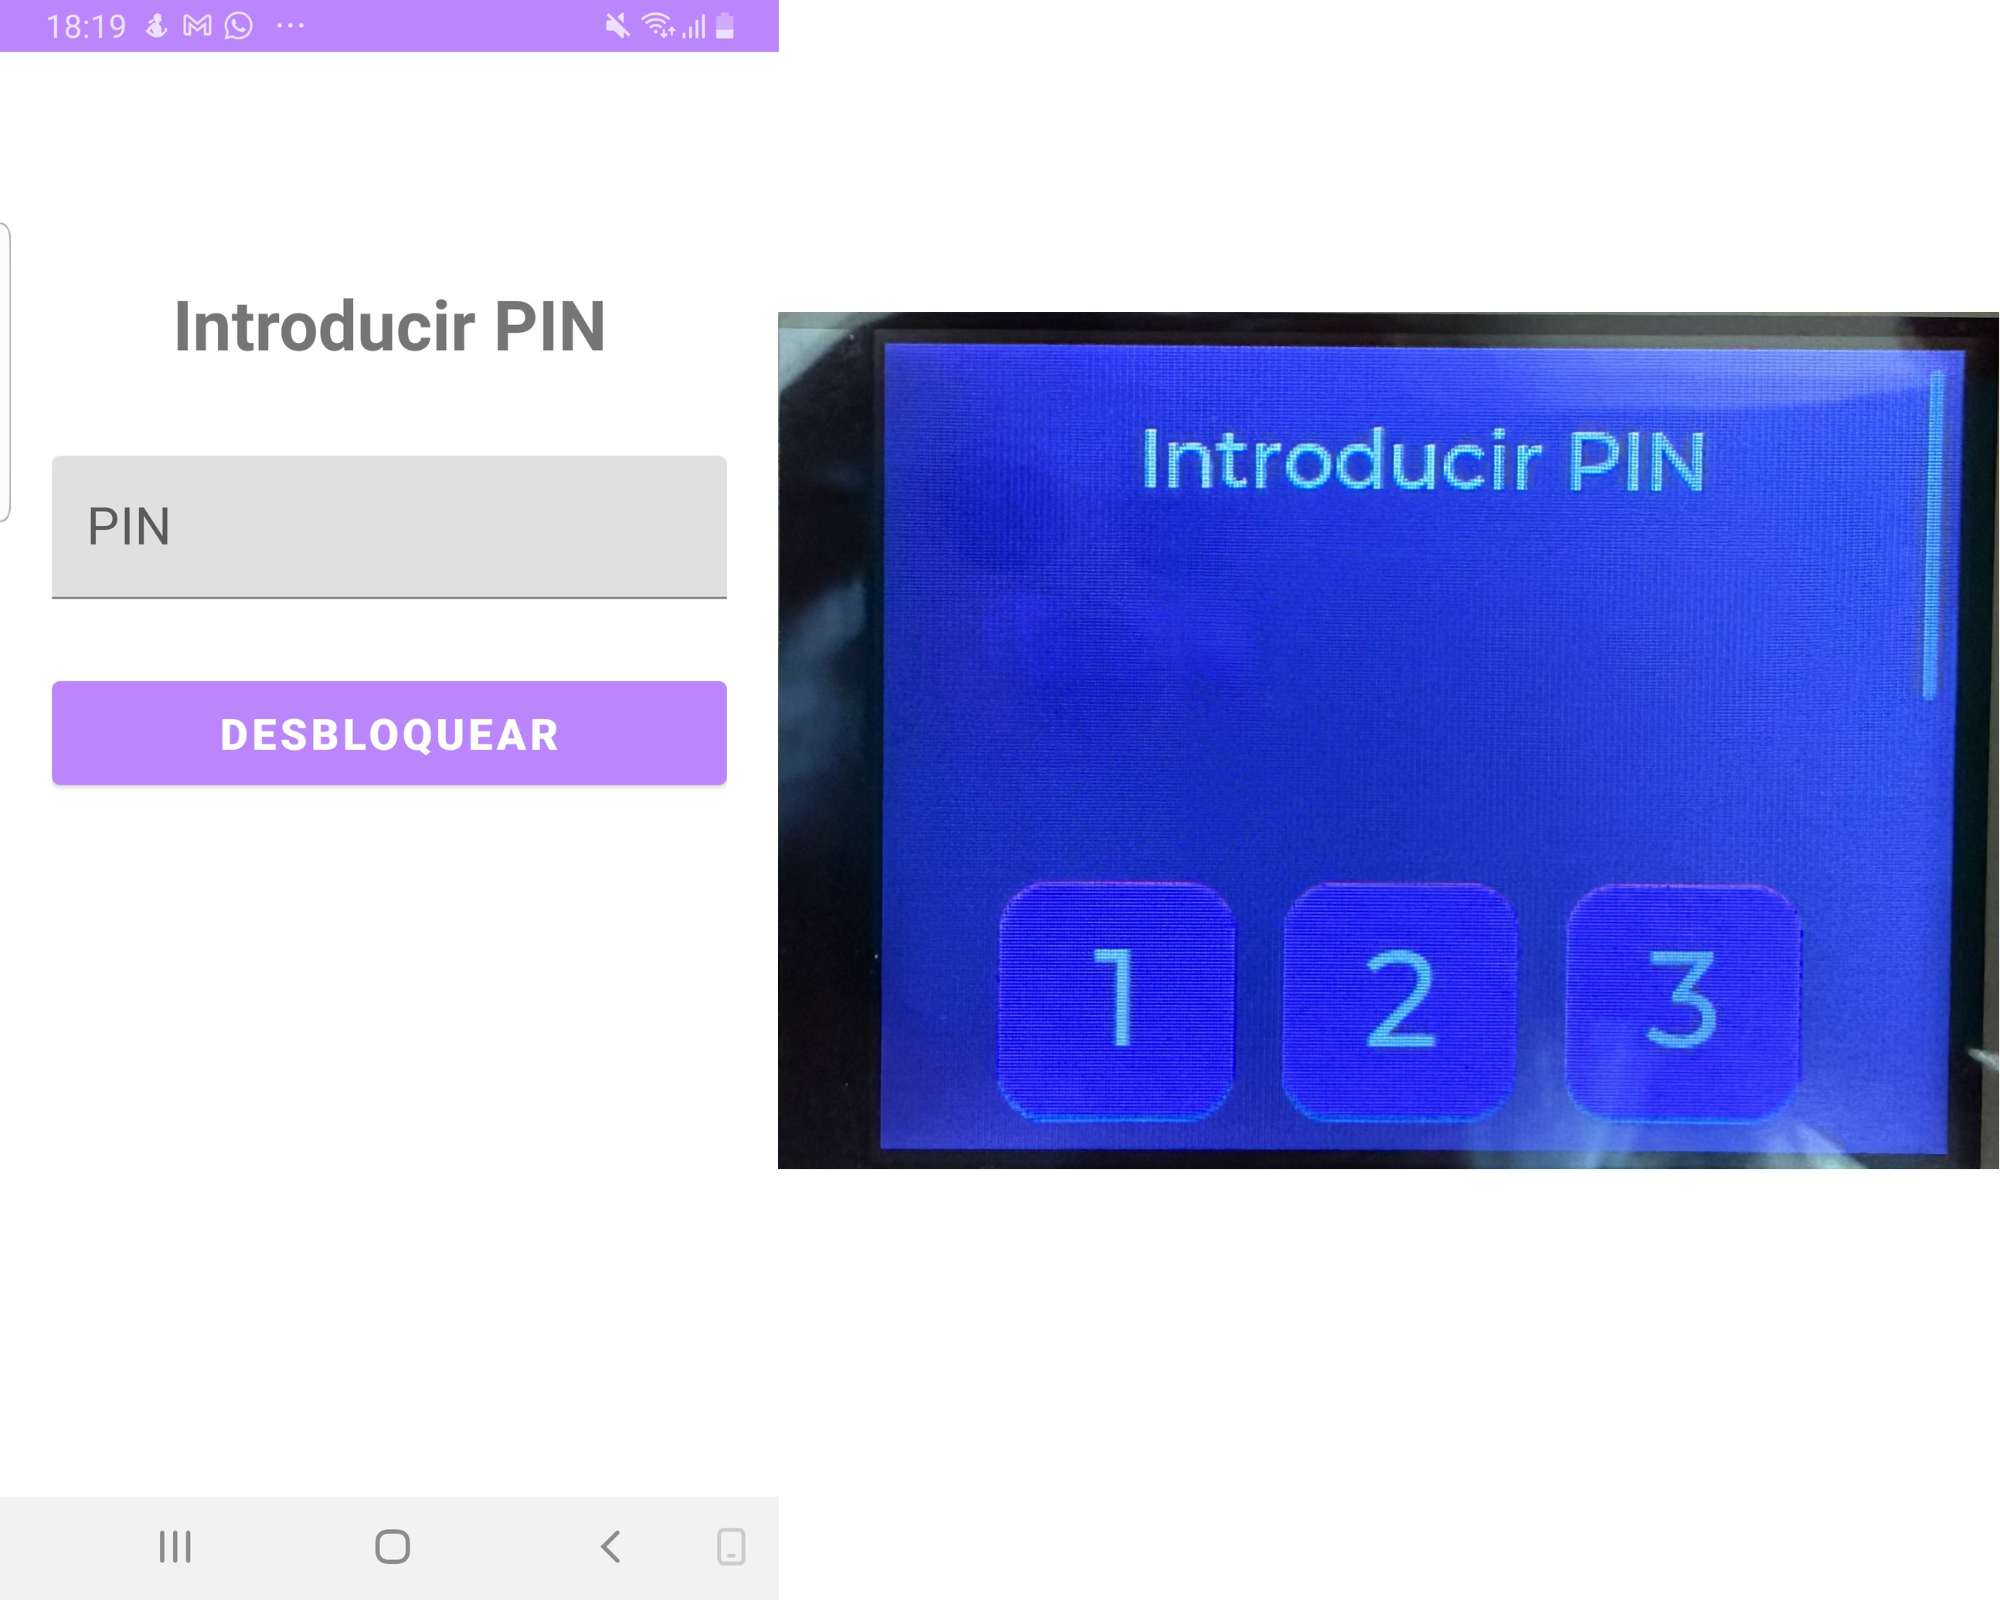
\includegraphics[width=0.85\textwidth]{figs/collage_PIN.png}
    \caption{Pantallas de desbloqueo mediante PIN}
    \label{fig:manual_pin}
\end{figure}

Una vez introducido el PIN correcto, se concede acceso a todas sus funcionalidades.\\

En caso de introducir un PIN incorrecto, se mostrará un mensaje de error y permanecerá bloqueada hasta que se introduzca un código válido.\\

El PIN de acceso se sincroniza automáticamente entre la app y el dispositivo. Cualquier modificación realizada desde uno de ellos será enviada al otro para mantener el mismo PIN actualizado en ambos. De esta forma ambos comparten un mismo PIN de 4 dígitos incluso en caso de reinicio, corte de corriente o pérdida de datos.\\

\section{Configuración inicial del dispositivo}

La primera vez que se utiliza el dispositivo, es necesario realizar un proceso de configuración inicial que permite conectarlo a la red WiFi y vincularlo con la aplicación móvil.\\

\textbf{Paso 1:} Conectar el teléfono móvil a la red WiFi generada por el dispositivo (\textit{MyMeds-Setup}).\\

\begin{figure}[H]
    \centering
    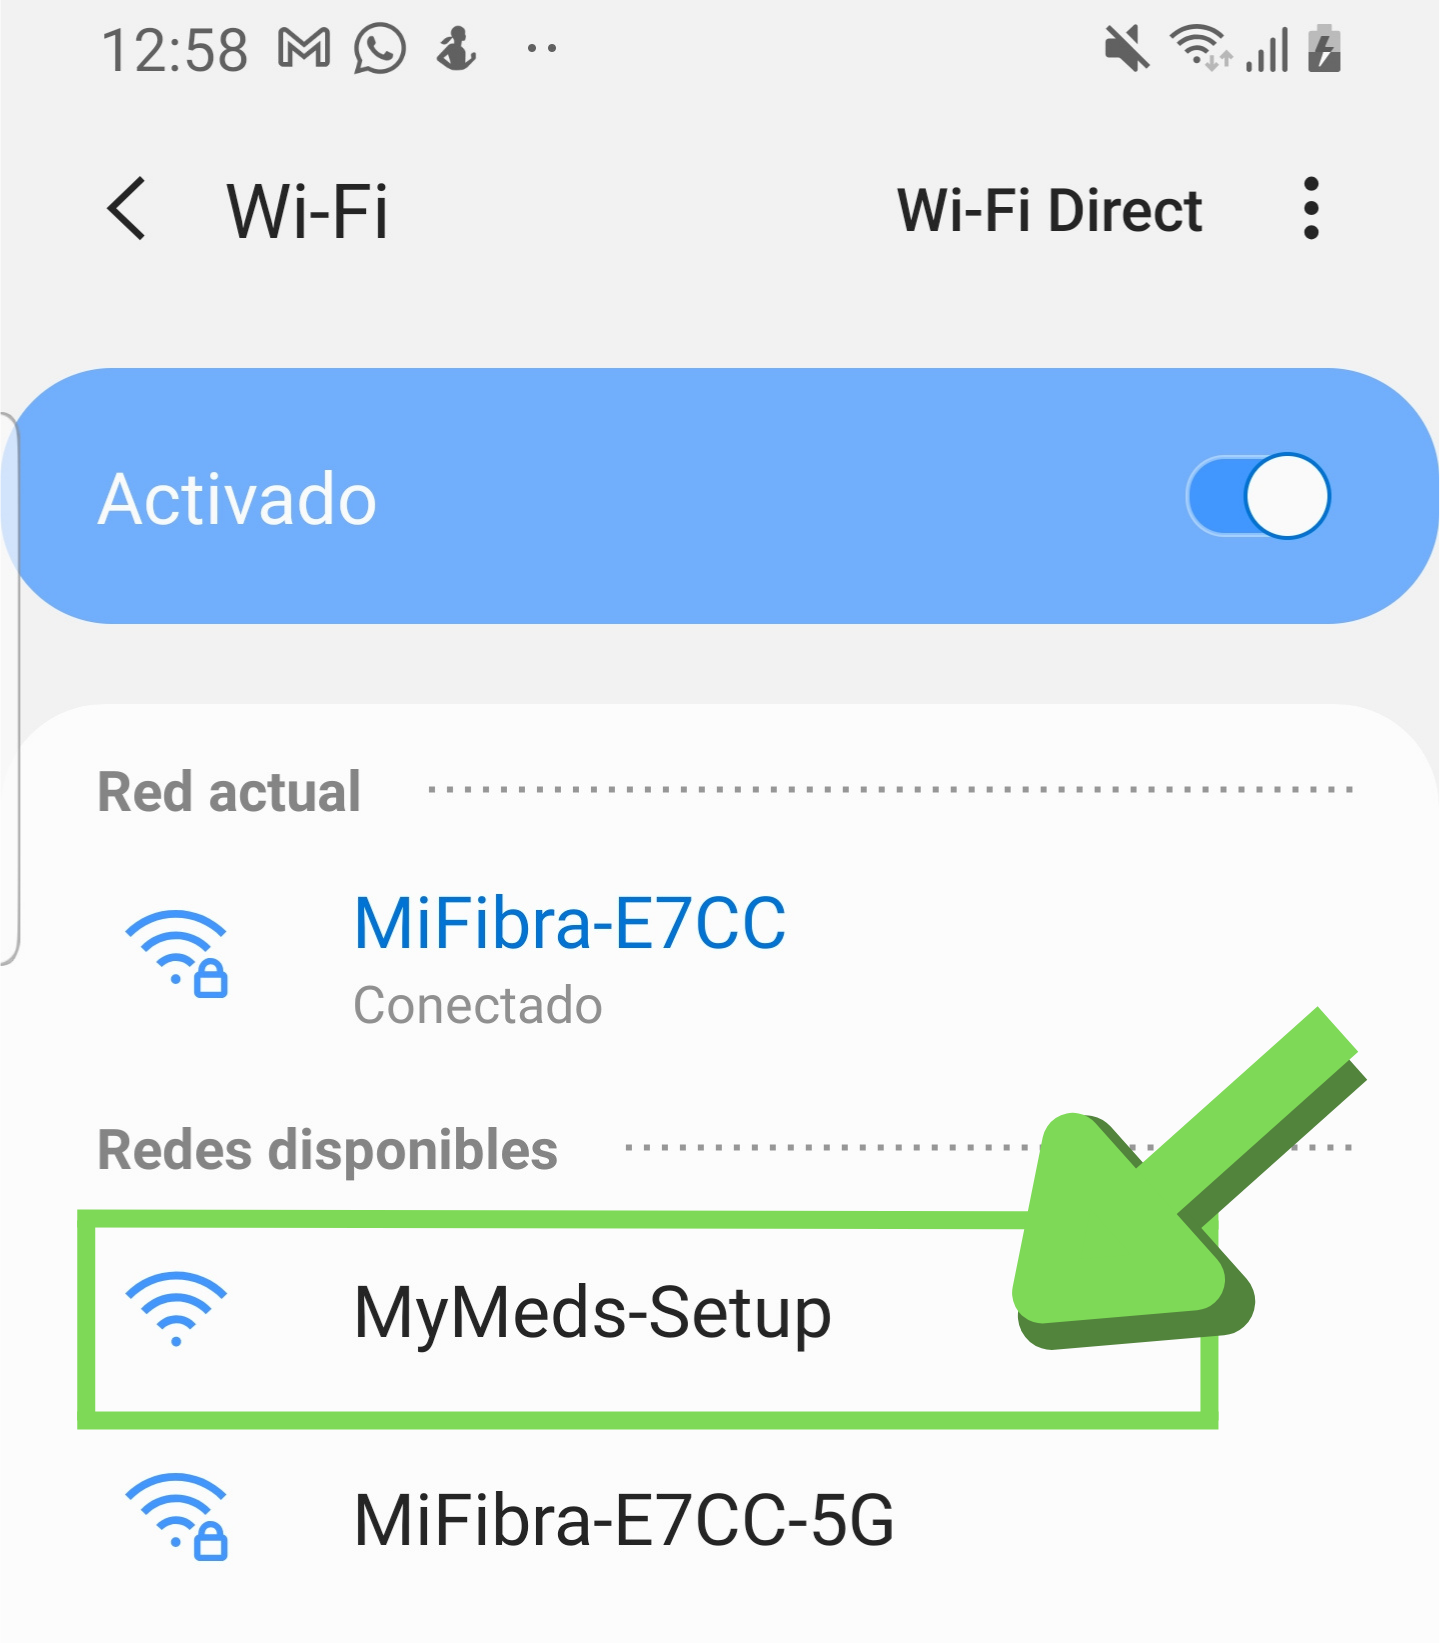
\includegraphics[width=0.45\textwidth]{figs/paso1_conf.png}
    \caption{Conectar red WiFi}
    \label{fig:paso1_conf}
\end{figure}

\

\

\textbf{Paso 2:} Abrir la aplicación móvil con el PIN 1234 y acceder al apartado \textit{Configurar dispensador}.\\

\begin{figure}[H]
    \centering
    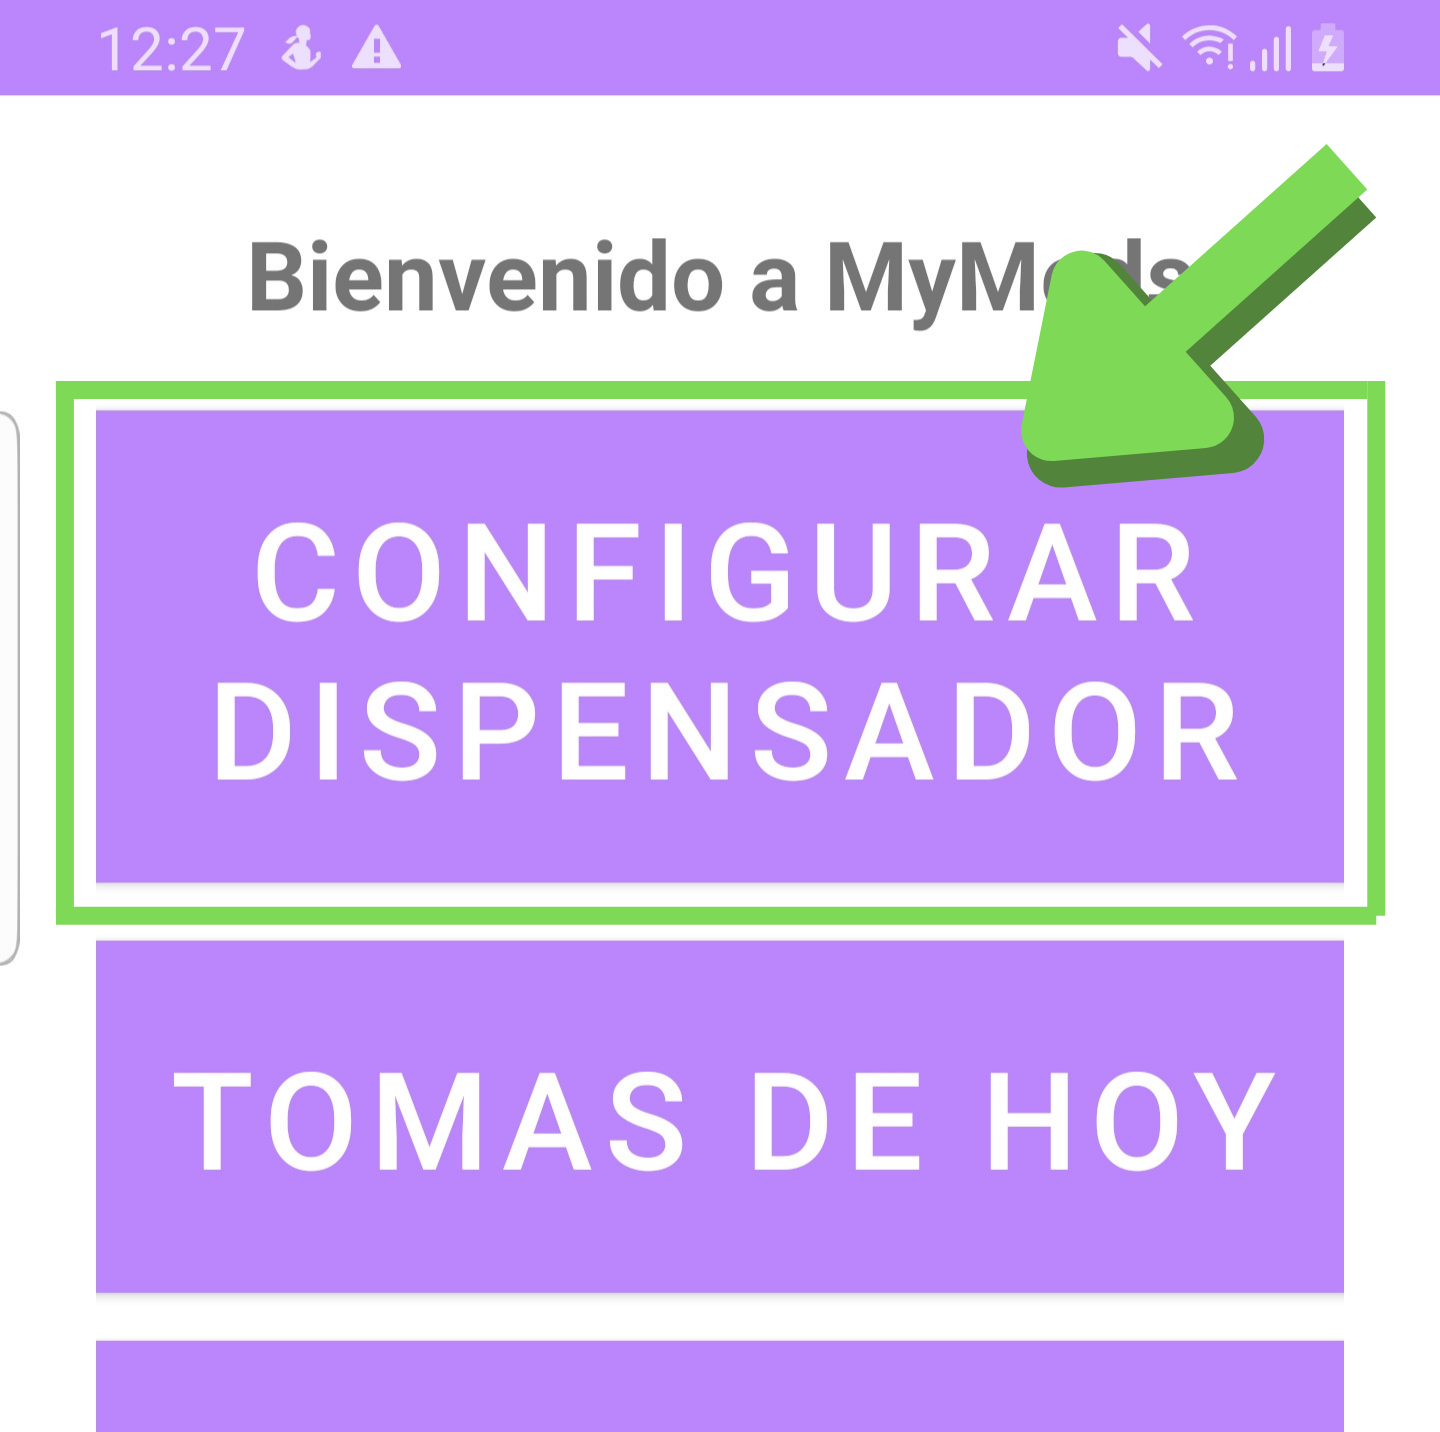
\includegraphics[width=0.45\textwidth]{figs/paso2_conf.png}
    \caption{Entrar a la configuración del dispensador}
    \label{fig:paso2_conf}
\end{figure}

\textbf{Paso 3:} Esperar a que la pantalla muestre que no  hay un dispositivo configurado y pulsar el botón \textit{Escanear QR}.\\


\begin{figure}[H]
    \centering
    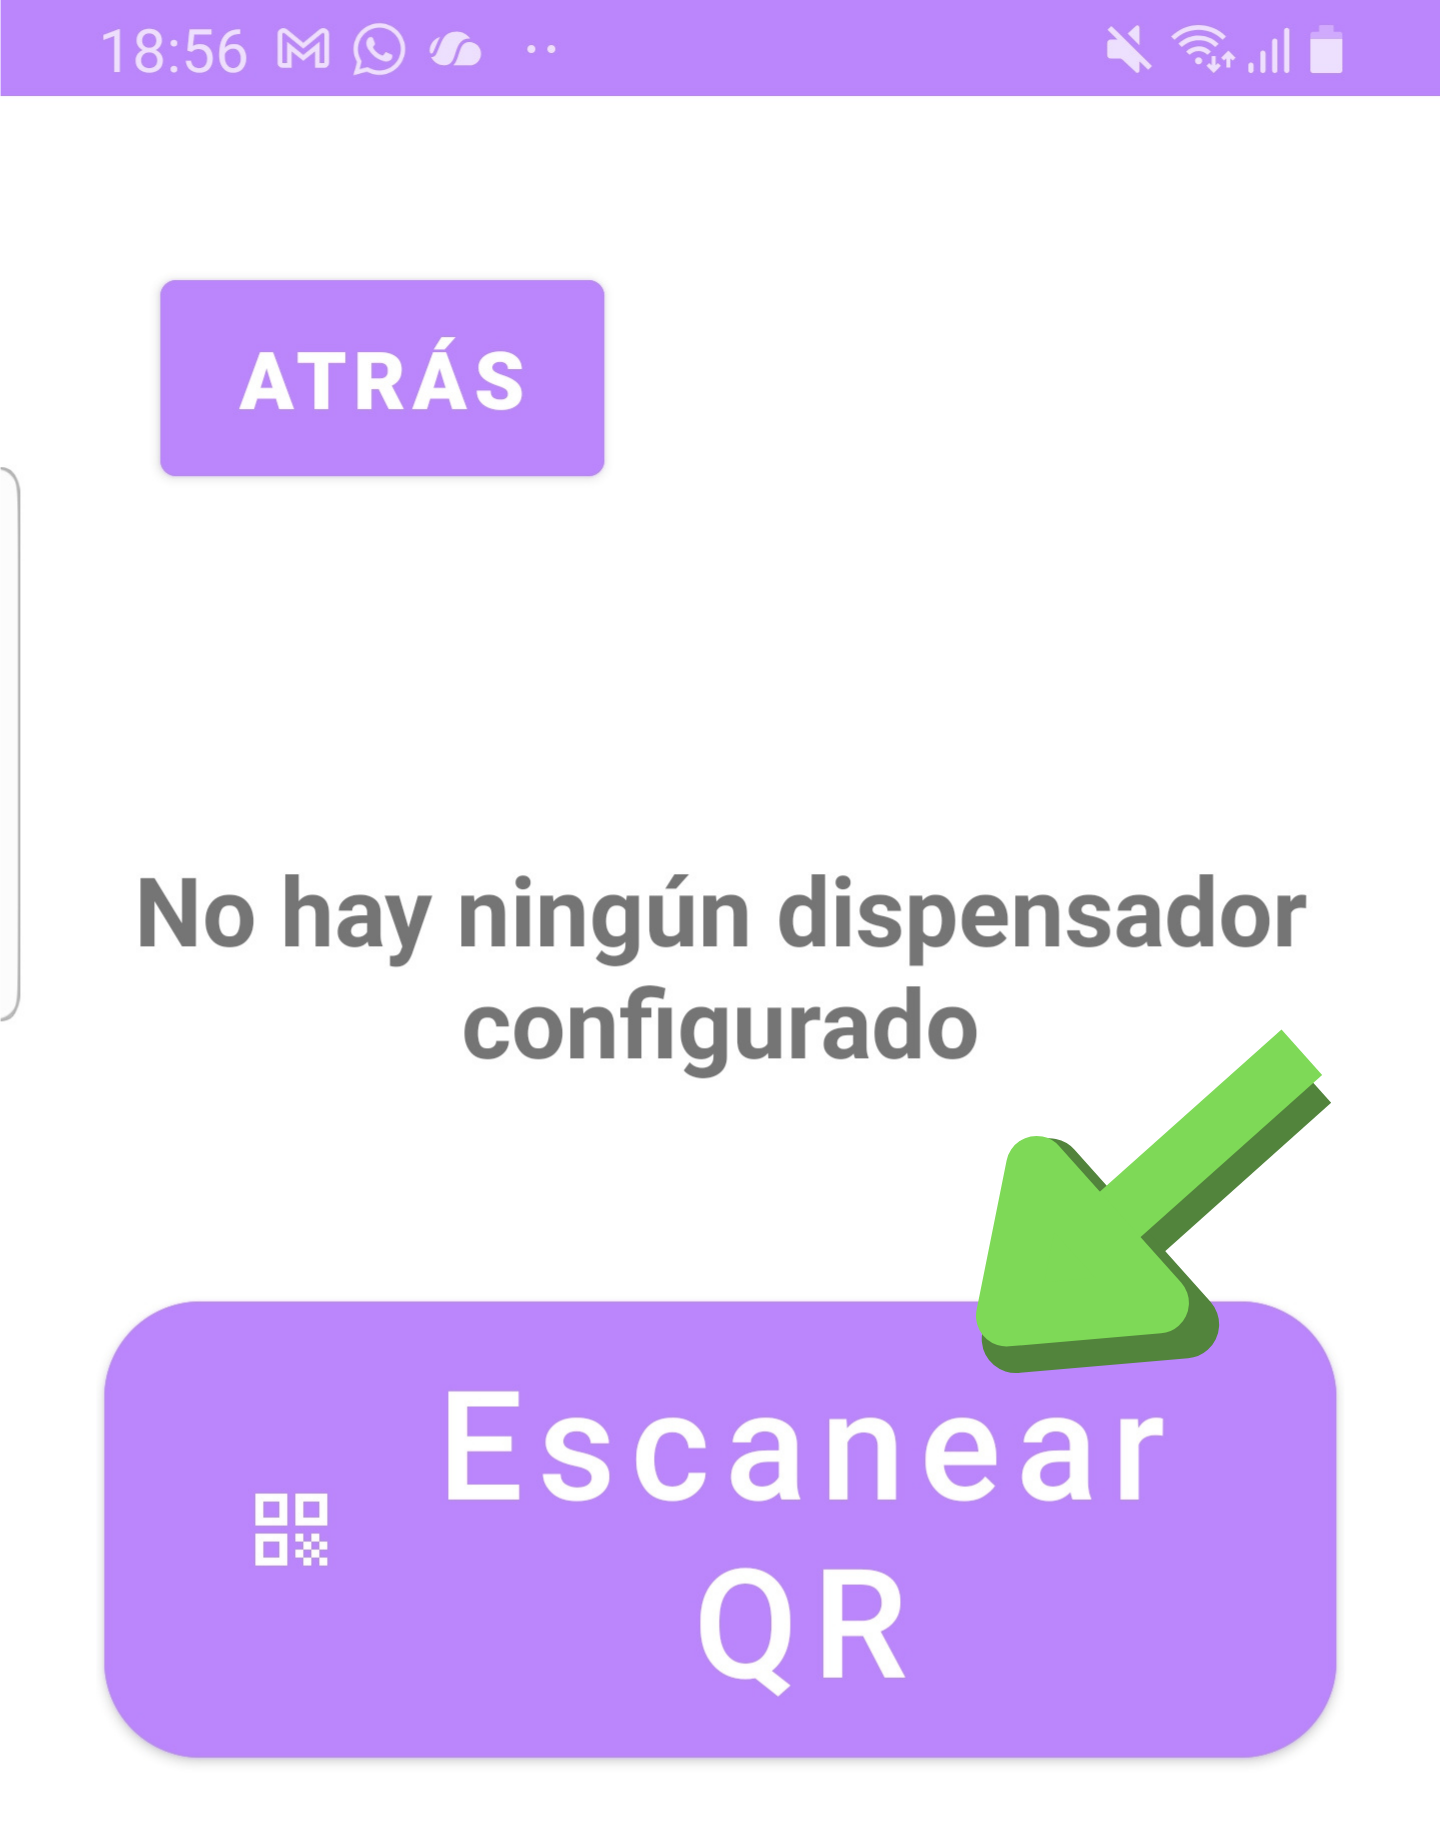
\includegraphics[width=0.45\textwidth]{figs/paso3_conf.png}
    \caption{Botón para abrir el escáner}
    \label{fig:paso3_conf}
\end{figure}

\

\

\textbf{Paso 4:} En la pantalla del dispositivo aparecerá un código QR que deberá ser escaneado desde la aplicación.\\

\begin{figure}[H]
    \centering
    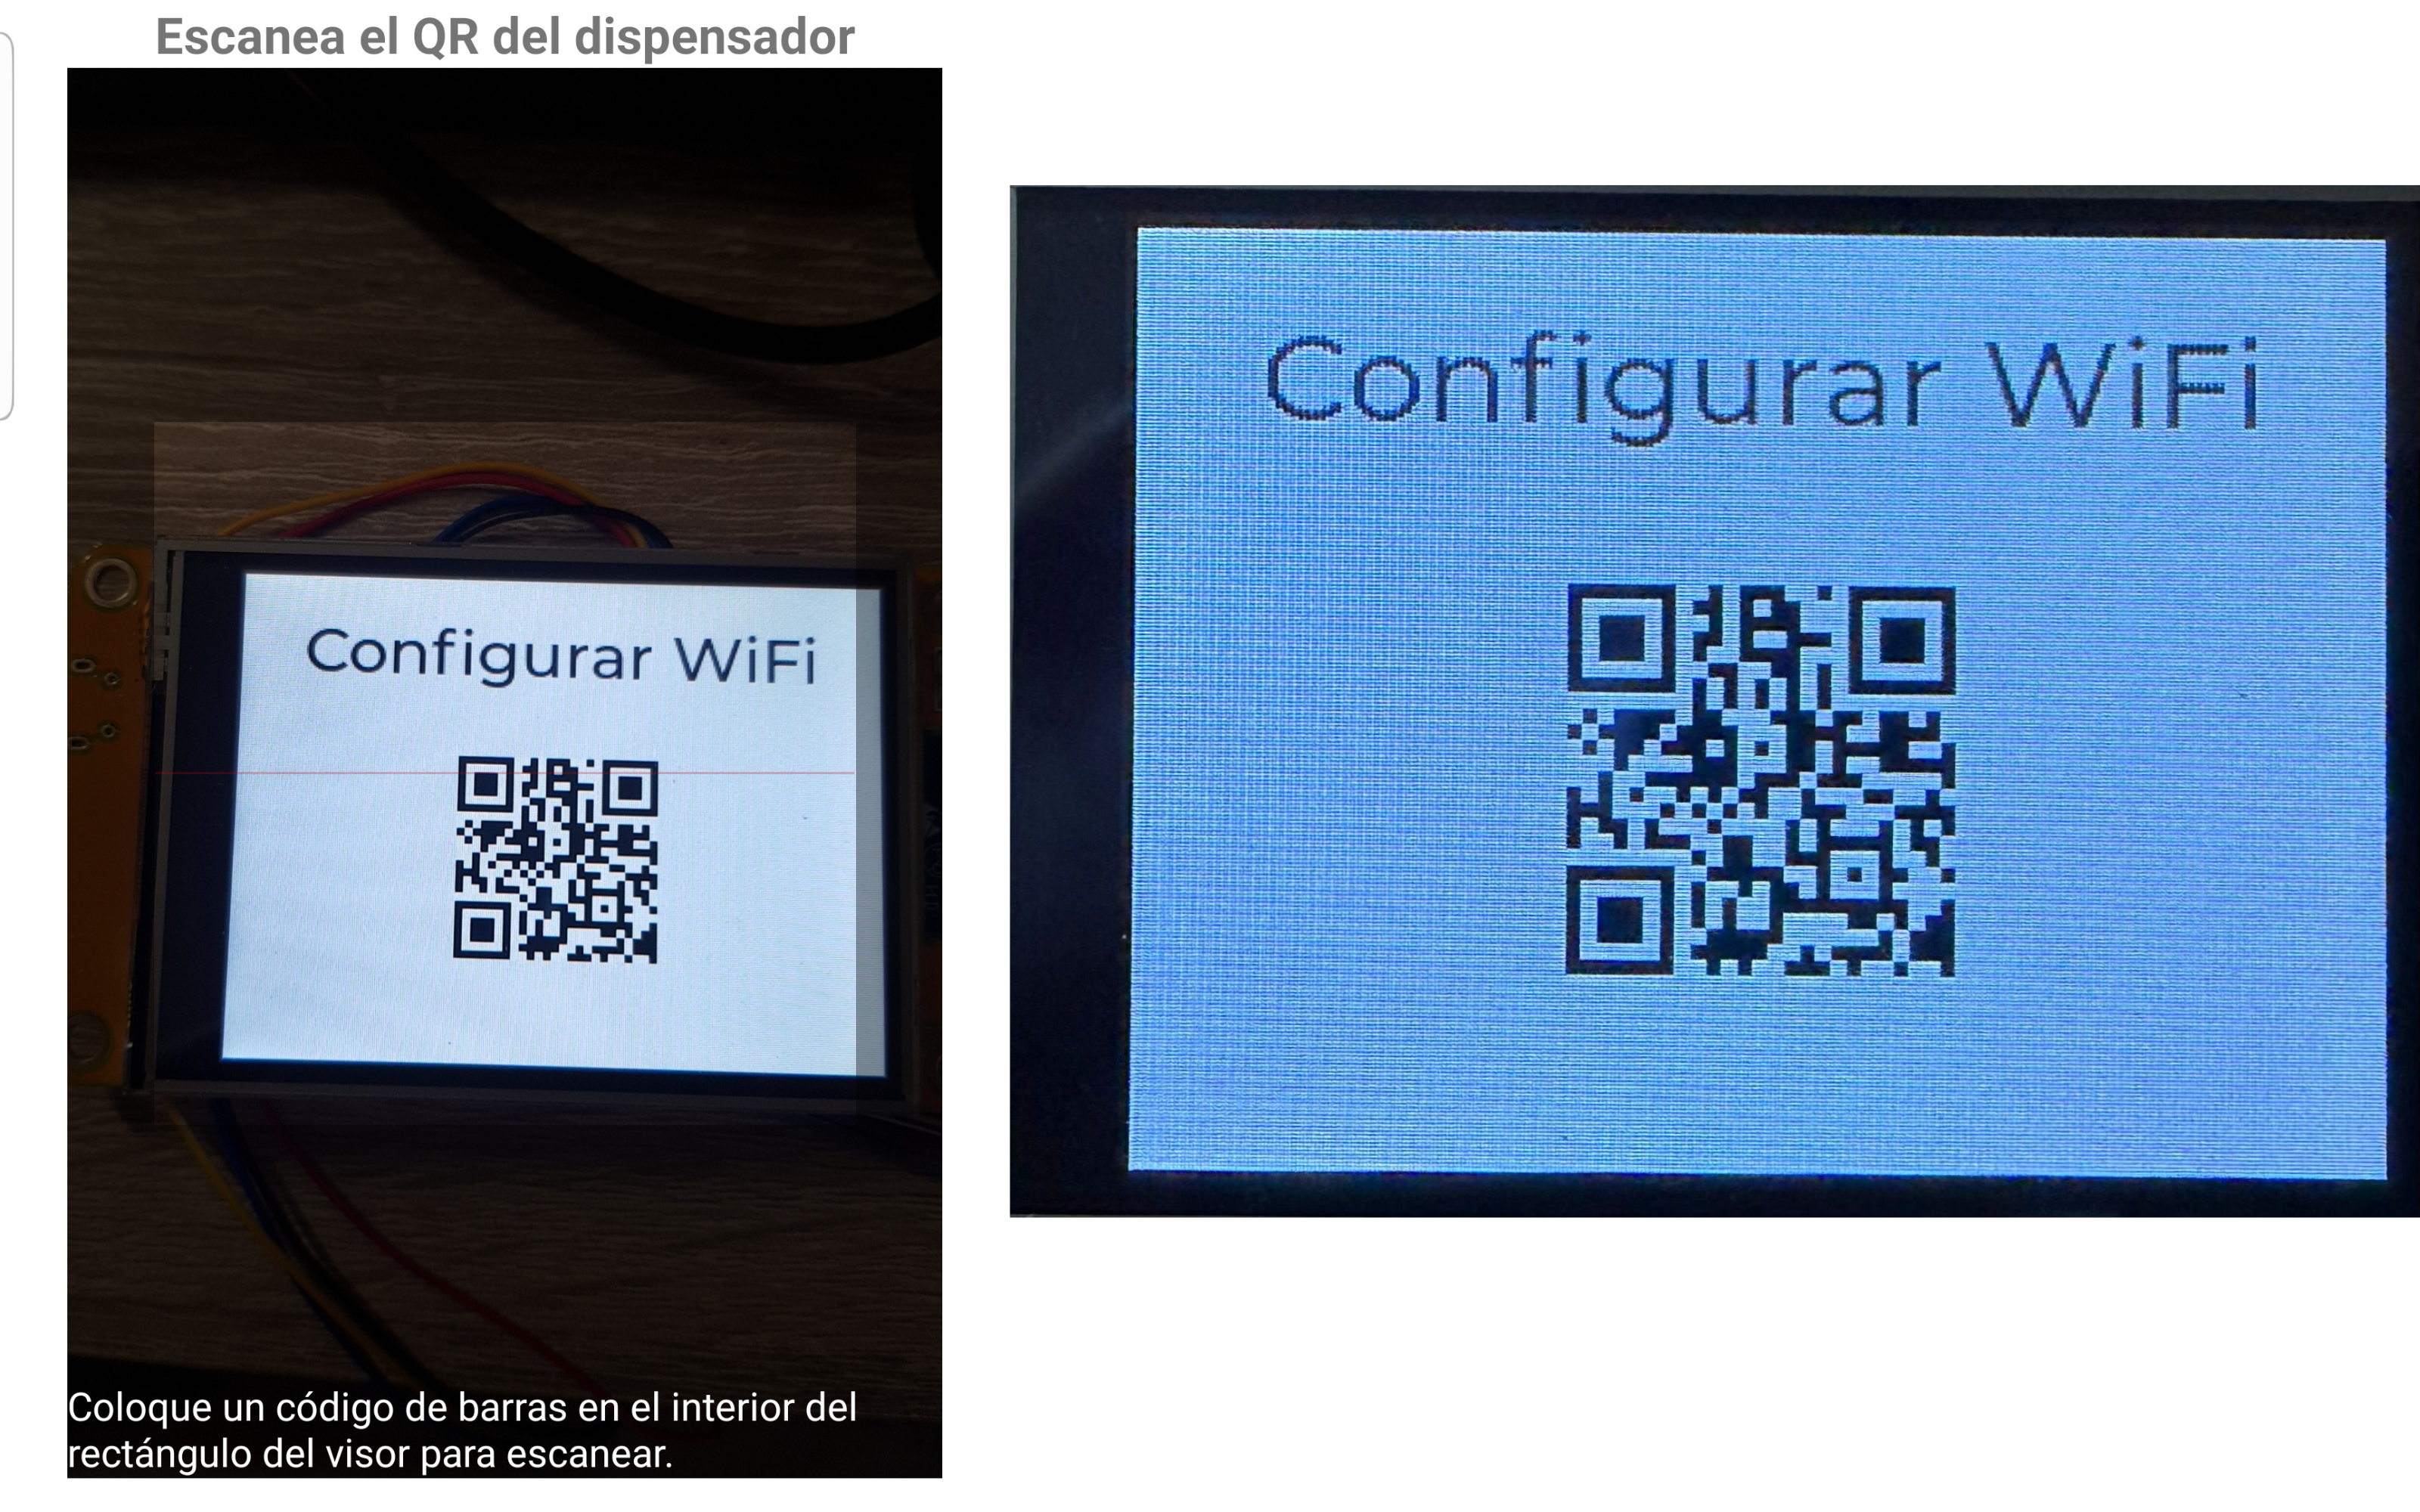
\includegraphics[width=0.8\textwidth]{figs/collage_paso4_conf.png}
    \caption{Ejemplo con QR que se muestra en el dispositivo}
    \label{fig:paso4_conf}
\end{figure}

\textbf{Paso 5:} Introducir las credenciales de la red WiFi (SSID y contraseña) donde se utilizará el dispositivo.\\

\begin{figure}[H]
    \centering
    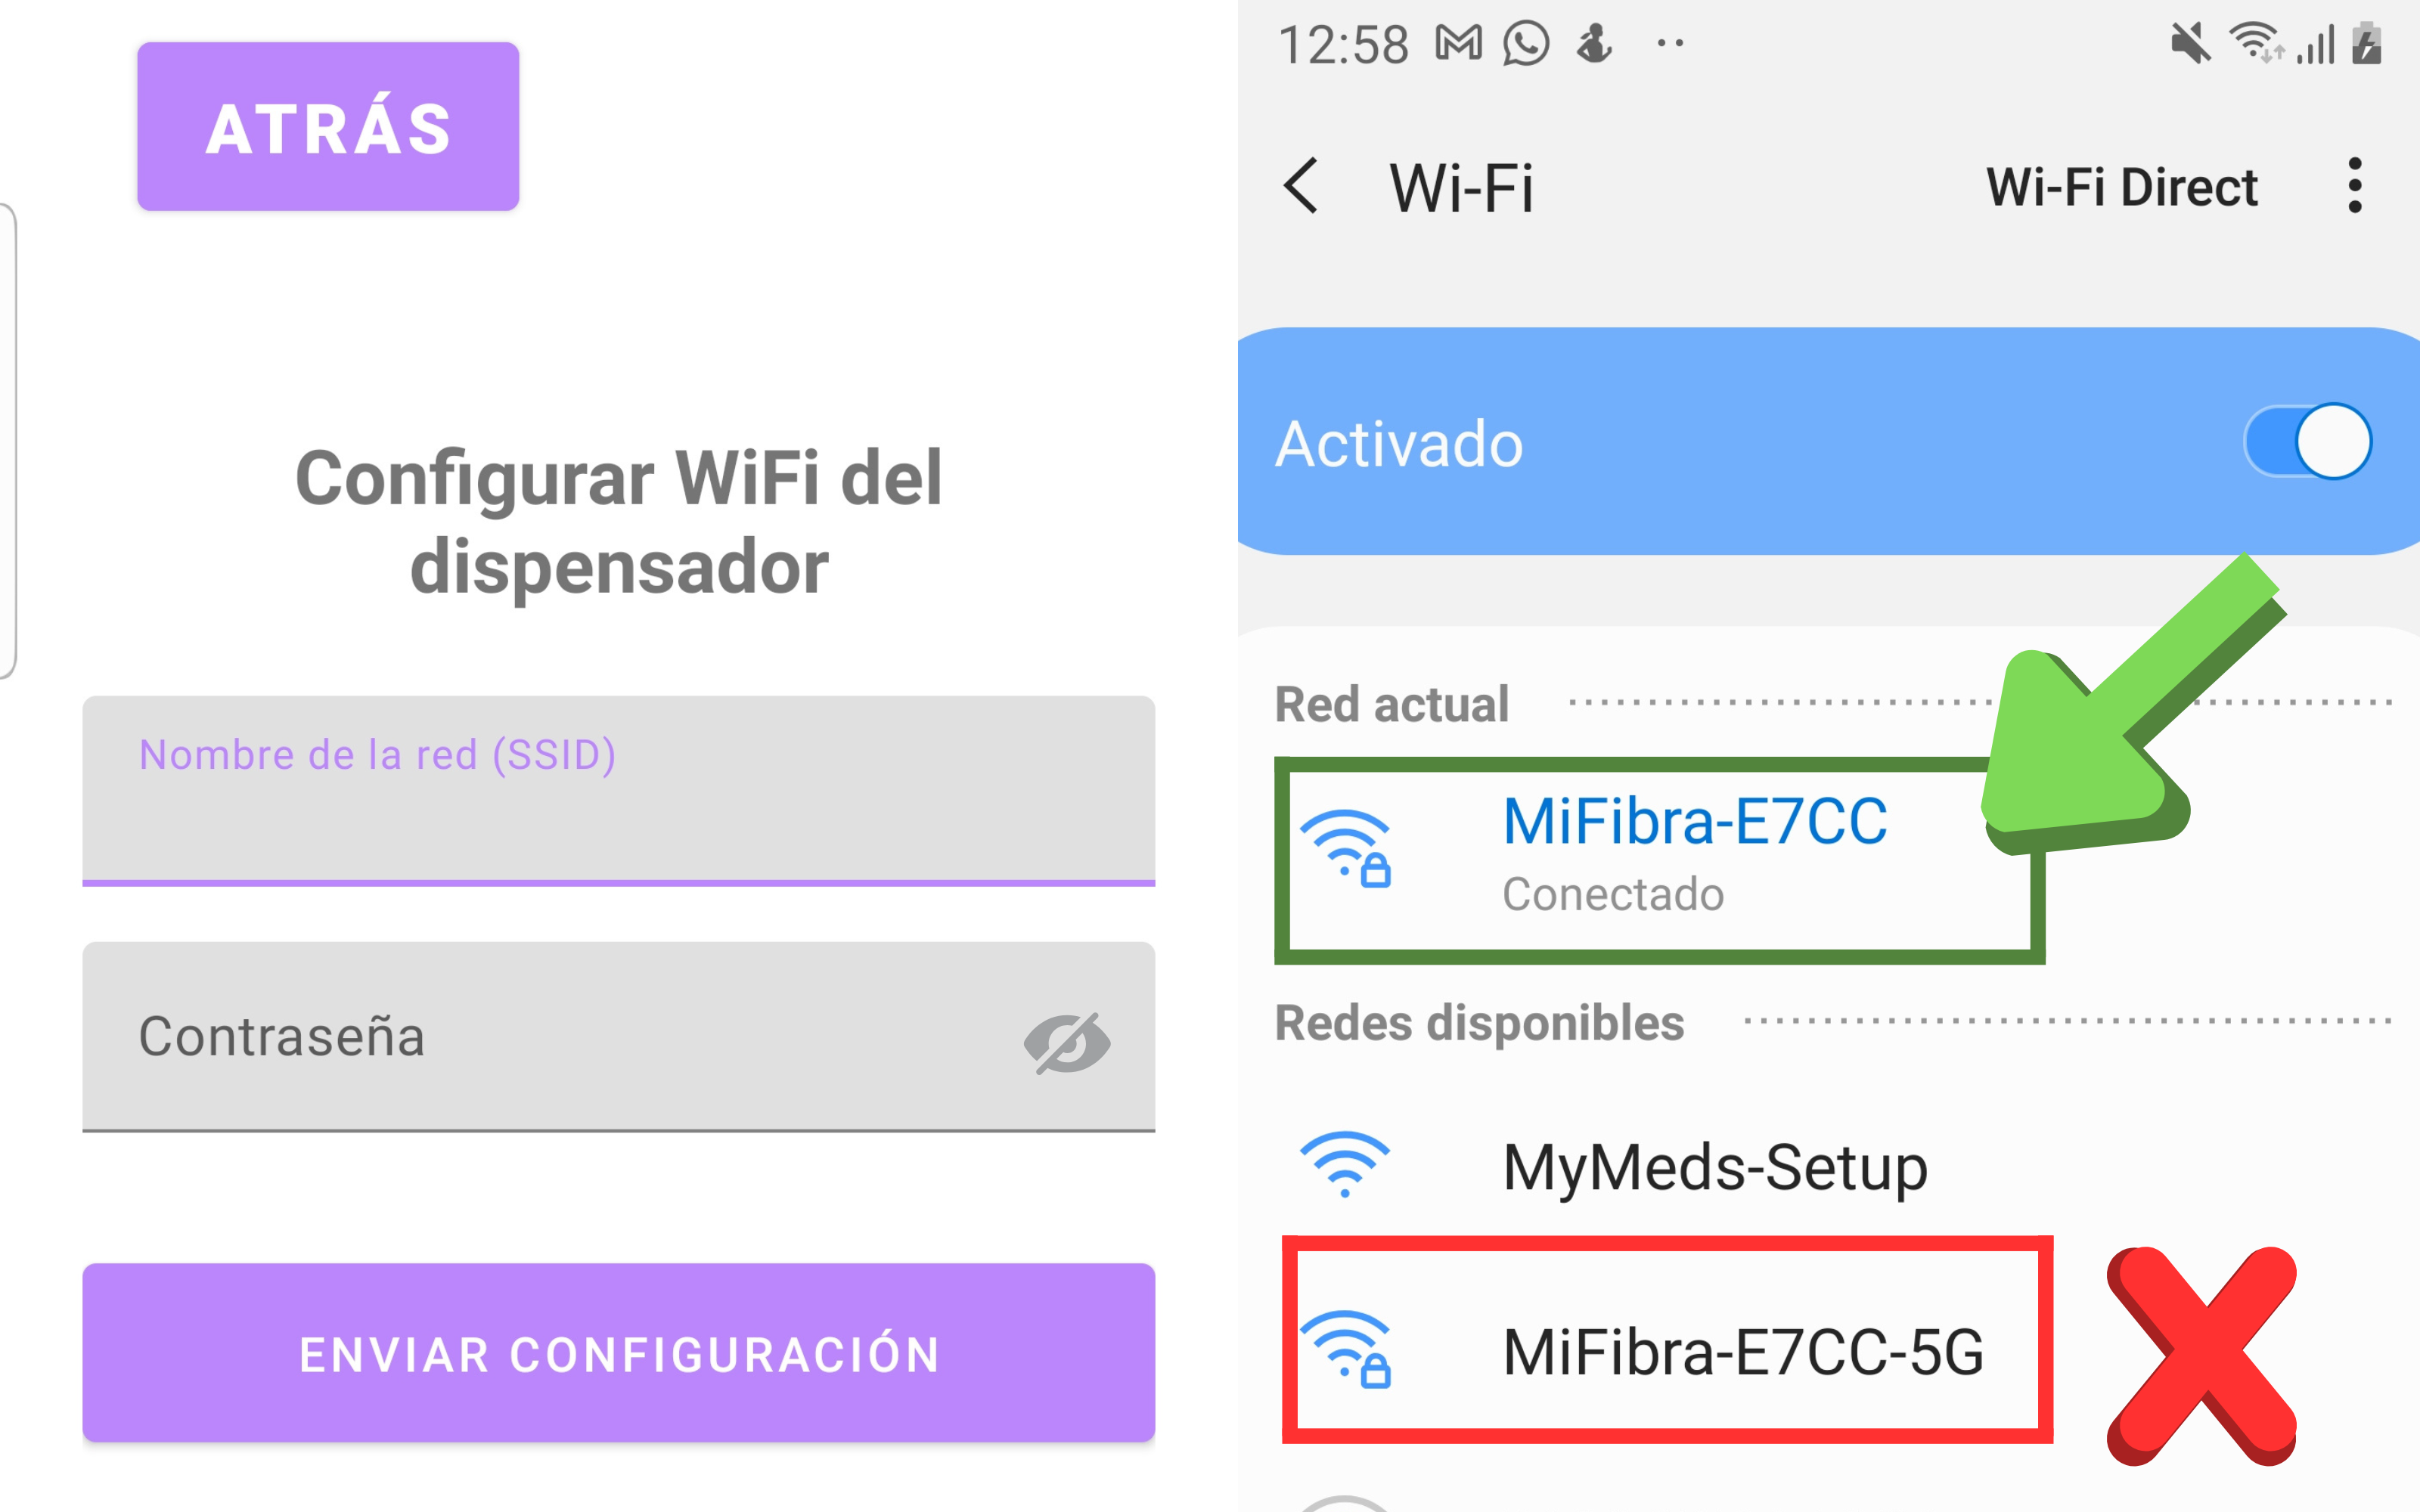
\includegraphics[width=0.8\textwidth]{figs/collage_paso5_conf.png}
    \caption{Introducir credenciales del WiFI}
    \label{fig:paso4_conf}
\end{figure}

\textit{Nota:} En caso de disponer de redes WiFi de 2.4 GHz y 5 GHz, se debe introducir la red de 2.4 GHz, ya que el dispositivo no es compatible con redes de 5 GHz.\\

\textbf{Paso 6:} Confirmar el envío de las credenciales. Durante este proceso, tanto la aplicación como el dispositivo indicarán que se está realizando la sincronización.\\


\textbf{Paso 7:} Esperar a que finalice el proceso de sincronización.\\

Una vez completada la configuración:

\begin{itemize}
    \item La aplicación mostrará la pantalla de configuración de tomas.
    \item El dispositivo pasará a la pantalla principal, donde se muestra la hora y el día de la semana.
\end{itemize}


\begin{figure}[H]
    \centering
    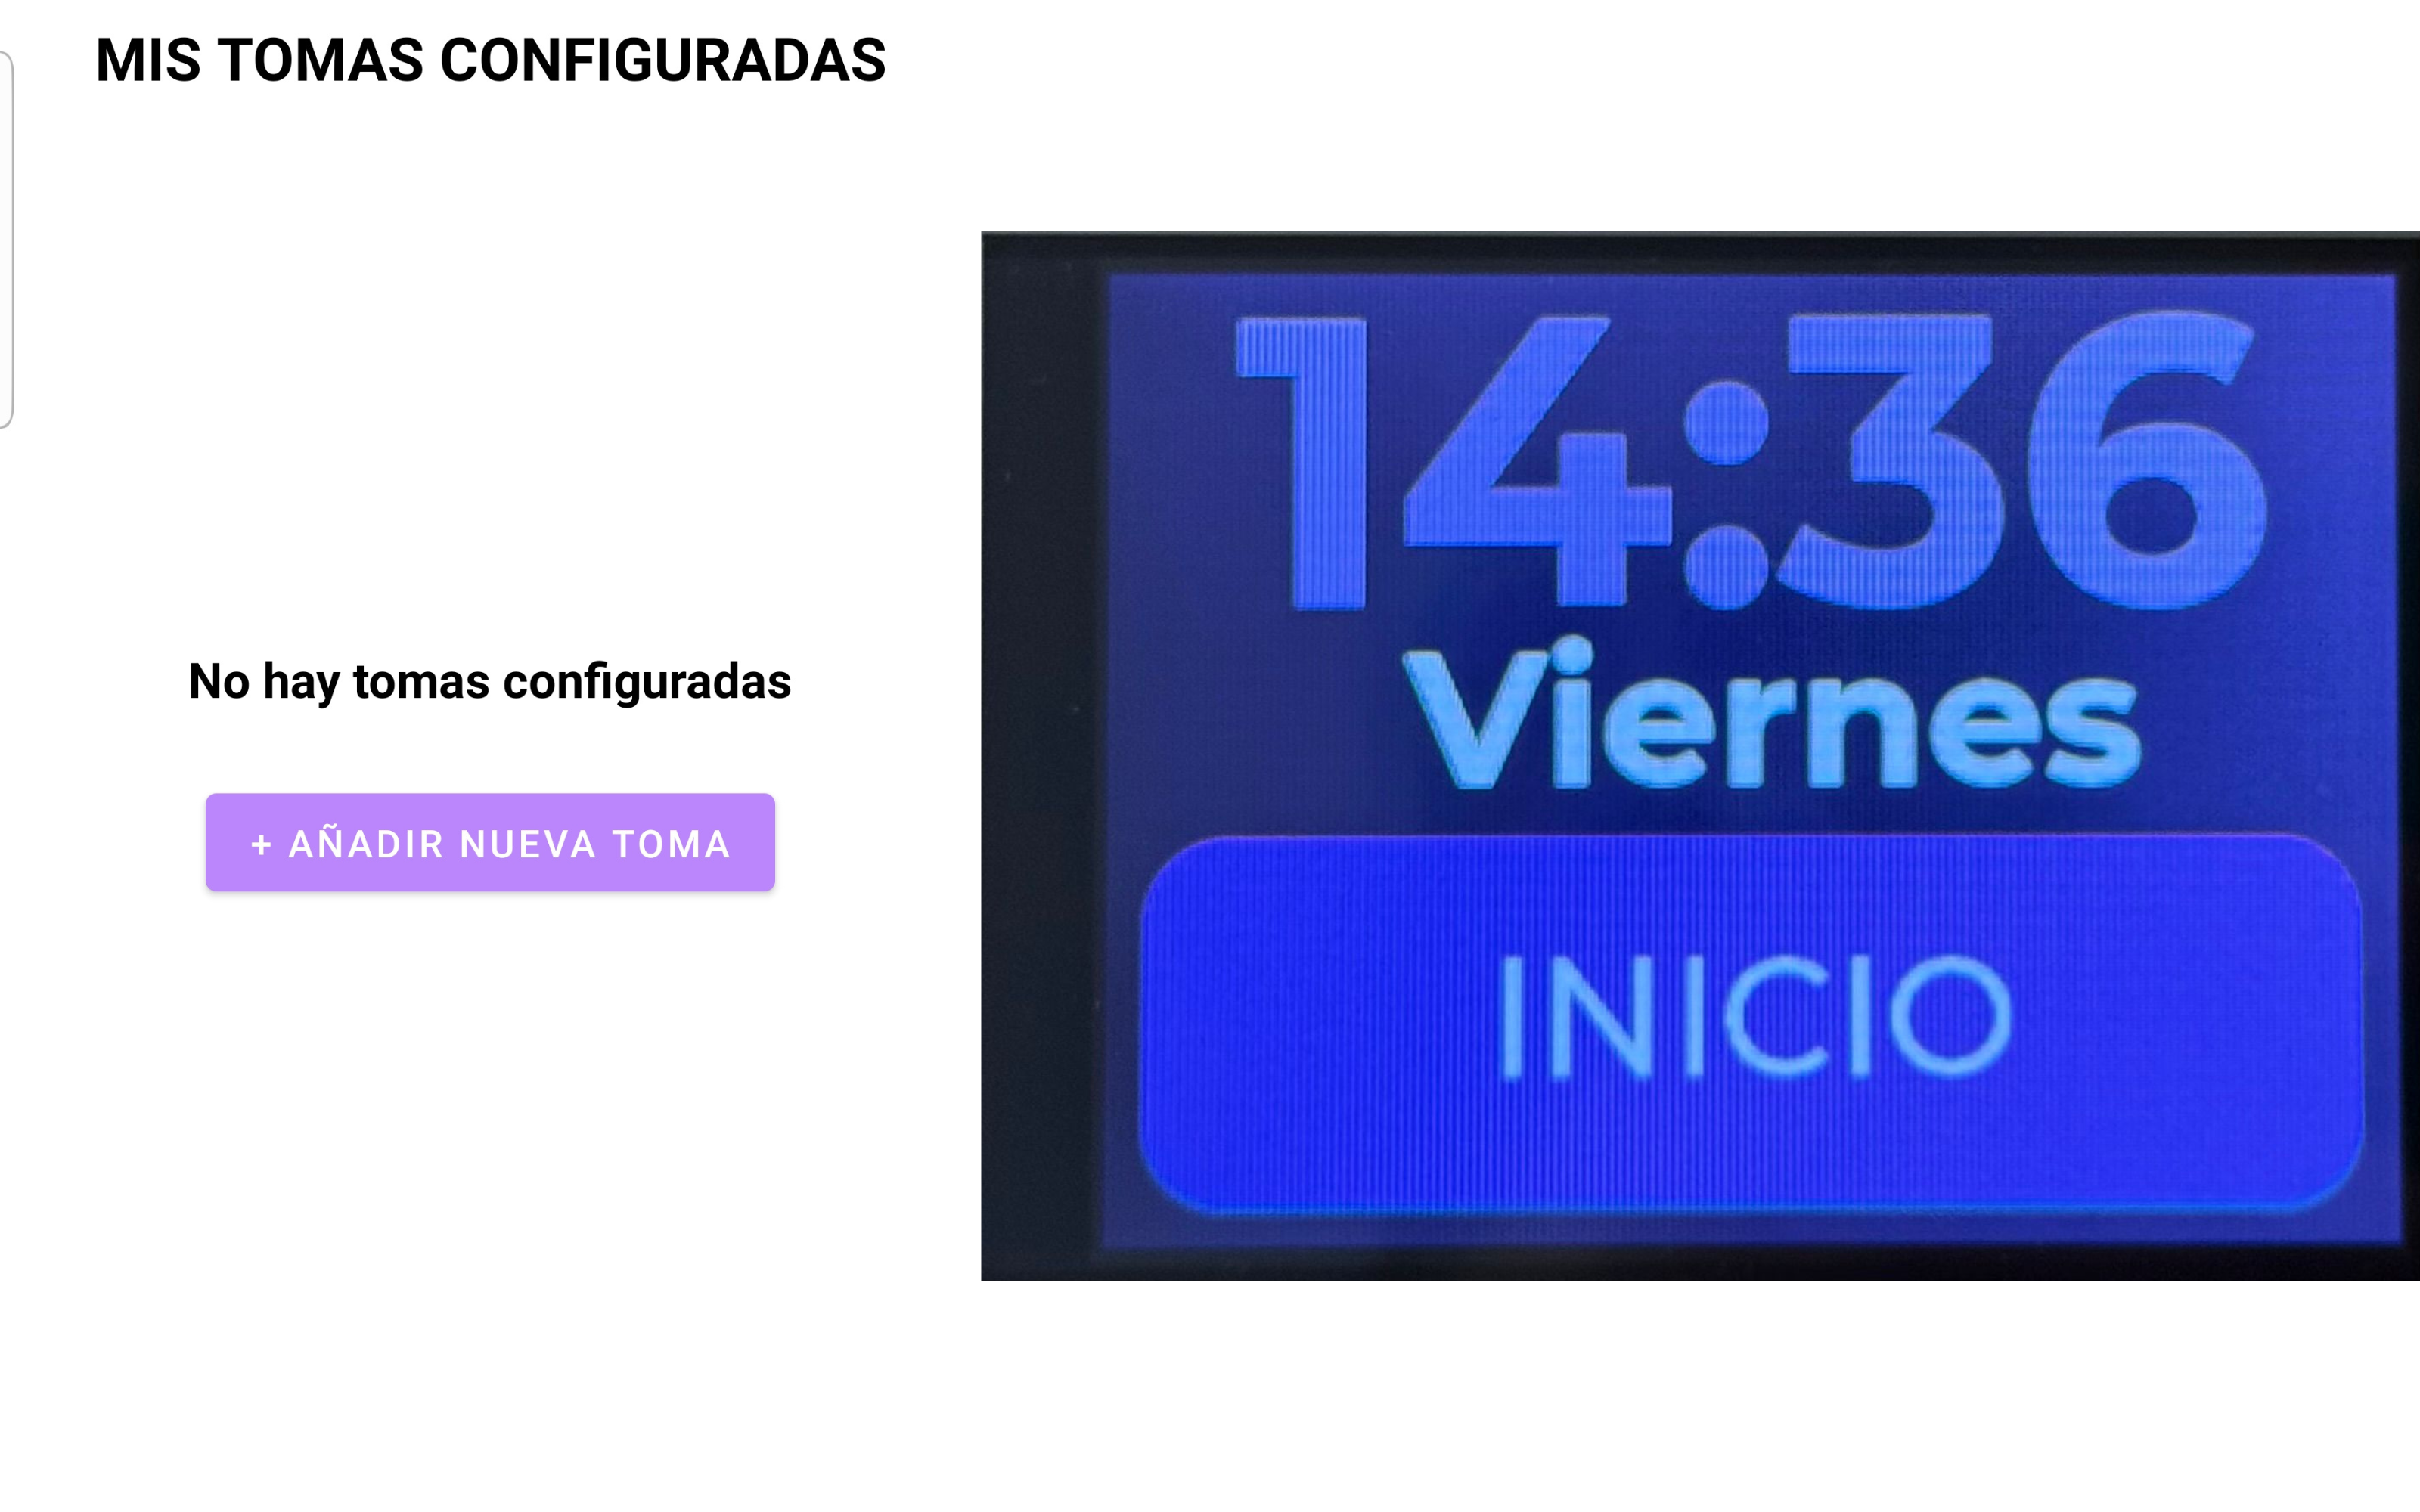
\includegraphics[width=0.85\textwidth]{figs/collage_paso7_conf.png}
    \caption{Pantallas que aparecen tras finalizar la sincronización}
    \label{fig:paso4_conf}
\end{figure}

\section{Descripción del dispositivo}

El dispositivo es un pastillero inteligente diseñado para facilitar la gestión diaria de la medicación mediante la automatización de las tomas, la emisión de recordatorios y la integración con una aplicación móvil.\\

Además de las funciones de dispensación, el sistema incorpora capacidades de monitorización biomédica y almacenamiento de información, permitiendo centralizar en un único dispositivo diferentes funcionalidades relacionadas con el seguimiento del usuario.\\

El dispositivo incorpora los siguientes elementos:

\begin{itemize}
\item Pantalla táctil para la interacción directa con el sistema.
\item Sistema automático de dispensación de medicación.
\item Altavoz para la emisión de avisos acústicos.
\item Conectividad WiFi para la sincronización con la aplicación móvil.
\item Sistema de autenticación mediante PIN.
\item Sensor biomédico para la medición de la frecuencia cardíaca.
\item Tarjeta microSD para el almacenamiento local de datos e histórico de mediciones.
\item Integración con aplicación móvil para la configuración y gestión remota del dispositivo.
\end{itemize}

La información almacenada en la tarjeta microSD permite mantener un histórico local de las mediciones realizadas, mientras que la aplicación móvil proporciona herramientas adicionales de consulta, visualización y análisis de los datos sincronizados.

\section{Uso del dispositivo}

\subsection{Pantalla principal}

Desde la pantalla principal puedes acceder a:

\begin{itemize}
\item Configuración de tomas
\item Visualización de tomas del día
\item Pulsómetro
\item Historial de mediciones del pulsómetro (En la app está dentro de `Pulsómetro`)
\item Gestión de medicamentos del dispensador
\item Ajustes
\end{itemize}

\begin{figure}[H]
    \centering
    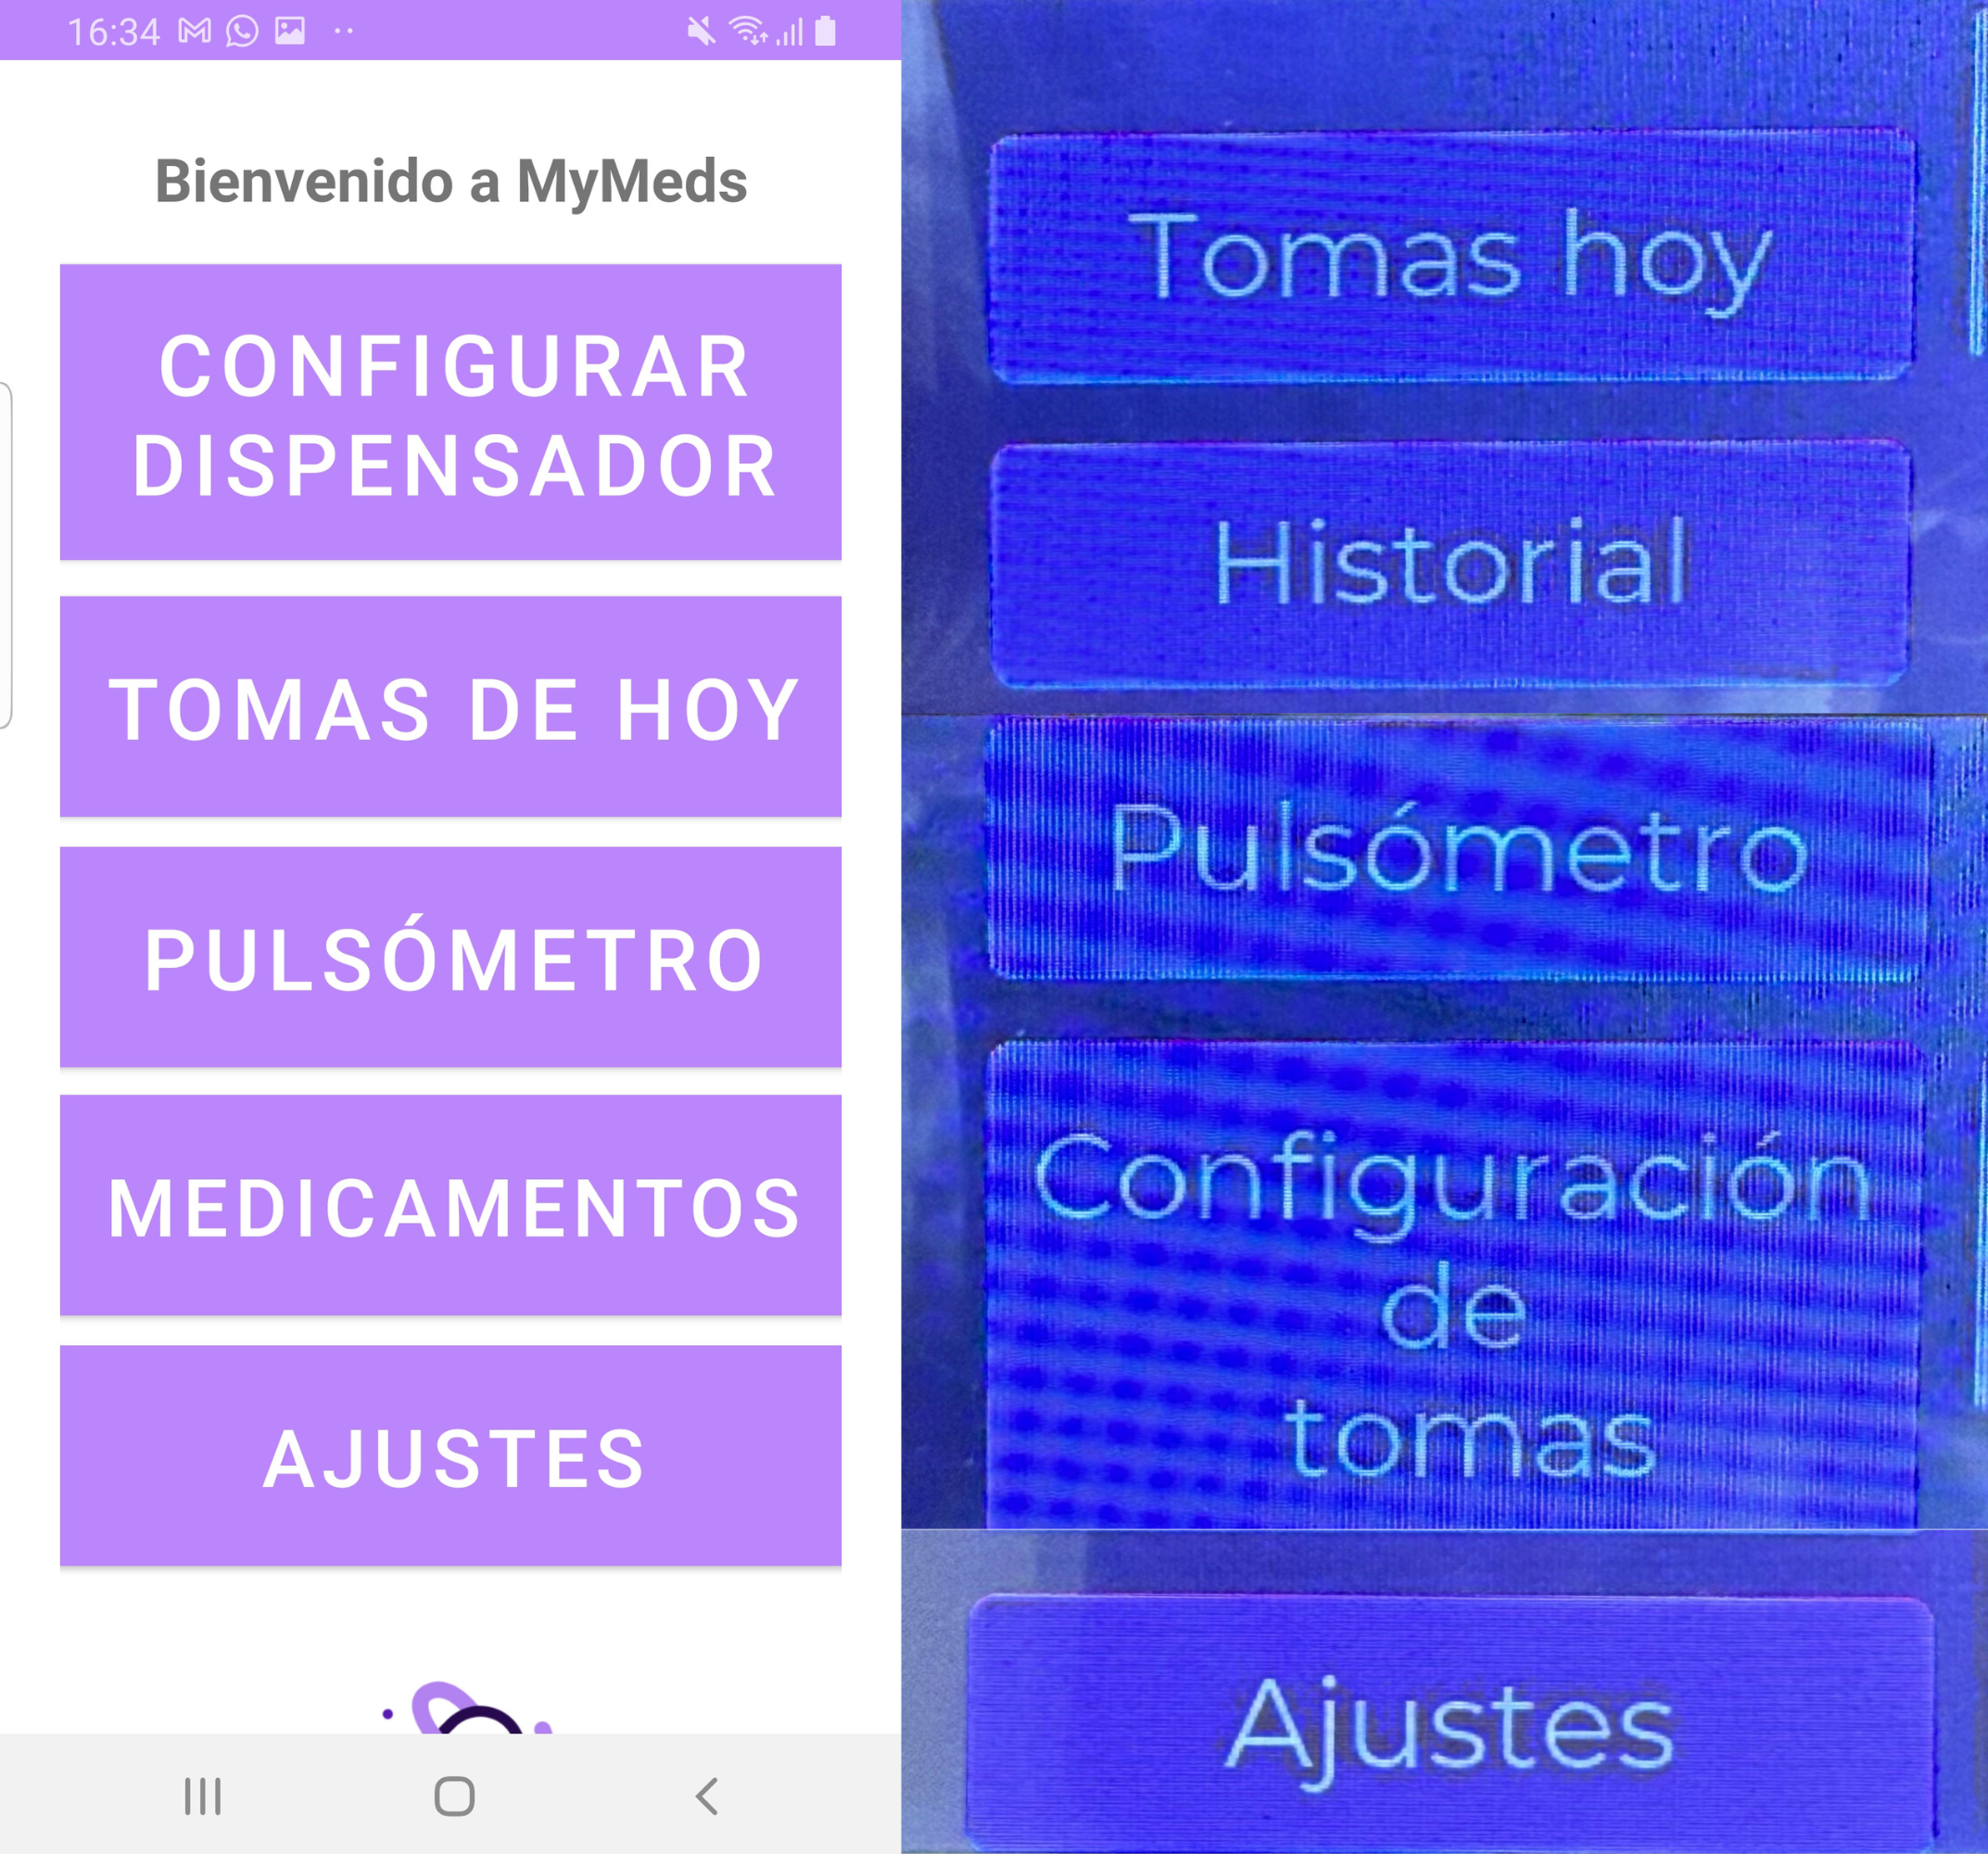
\includegraphics[width=0.85\textwidth]{figs/collage_pantallas_principales.png}
    \caption{Pantallas principales de la app y el dispositivo}
    \label{fig:pantallas_principales}
\end{figure}

La navegación se realiza mediante la pantalla táctil.

\subsection{Dispensación de medicación}

El dispositivo dispensa automáticamente la medicación en los horarios configurados.

Cuando llega la hora y día de una toma:

\begin{itemize}
\item Se activa una señal sonora
\item Se muestra un aviso en pantalla
\item Se dispensa la medicación correspondiente
\end{itemize}

Cada compartimento del sistema corresponde a una toma concreta.

\subsection{Avisos acústicos}

El dispositivo incorpora un altavoz que emite un aviso cuando es necesario alertar al usuario.\\

El sonido ha sido diseñado para ser:

\begin{itemize}
\item Claramente audible
\item Suave y no molesto
\item Adecuado para uso diario
\end{itemize}

Desde el apartado de `Ajustes`, será posible elegir entre 3 rangos de volumen para los avisos [Bajo - Medio - Alto].

\begin{figure}[H]
    \centering
    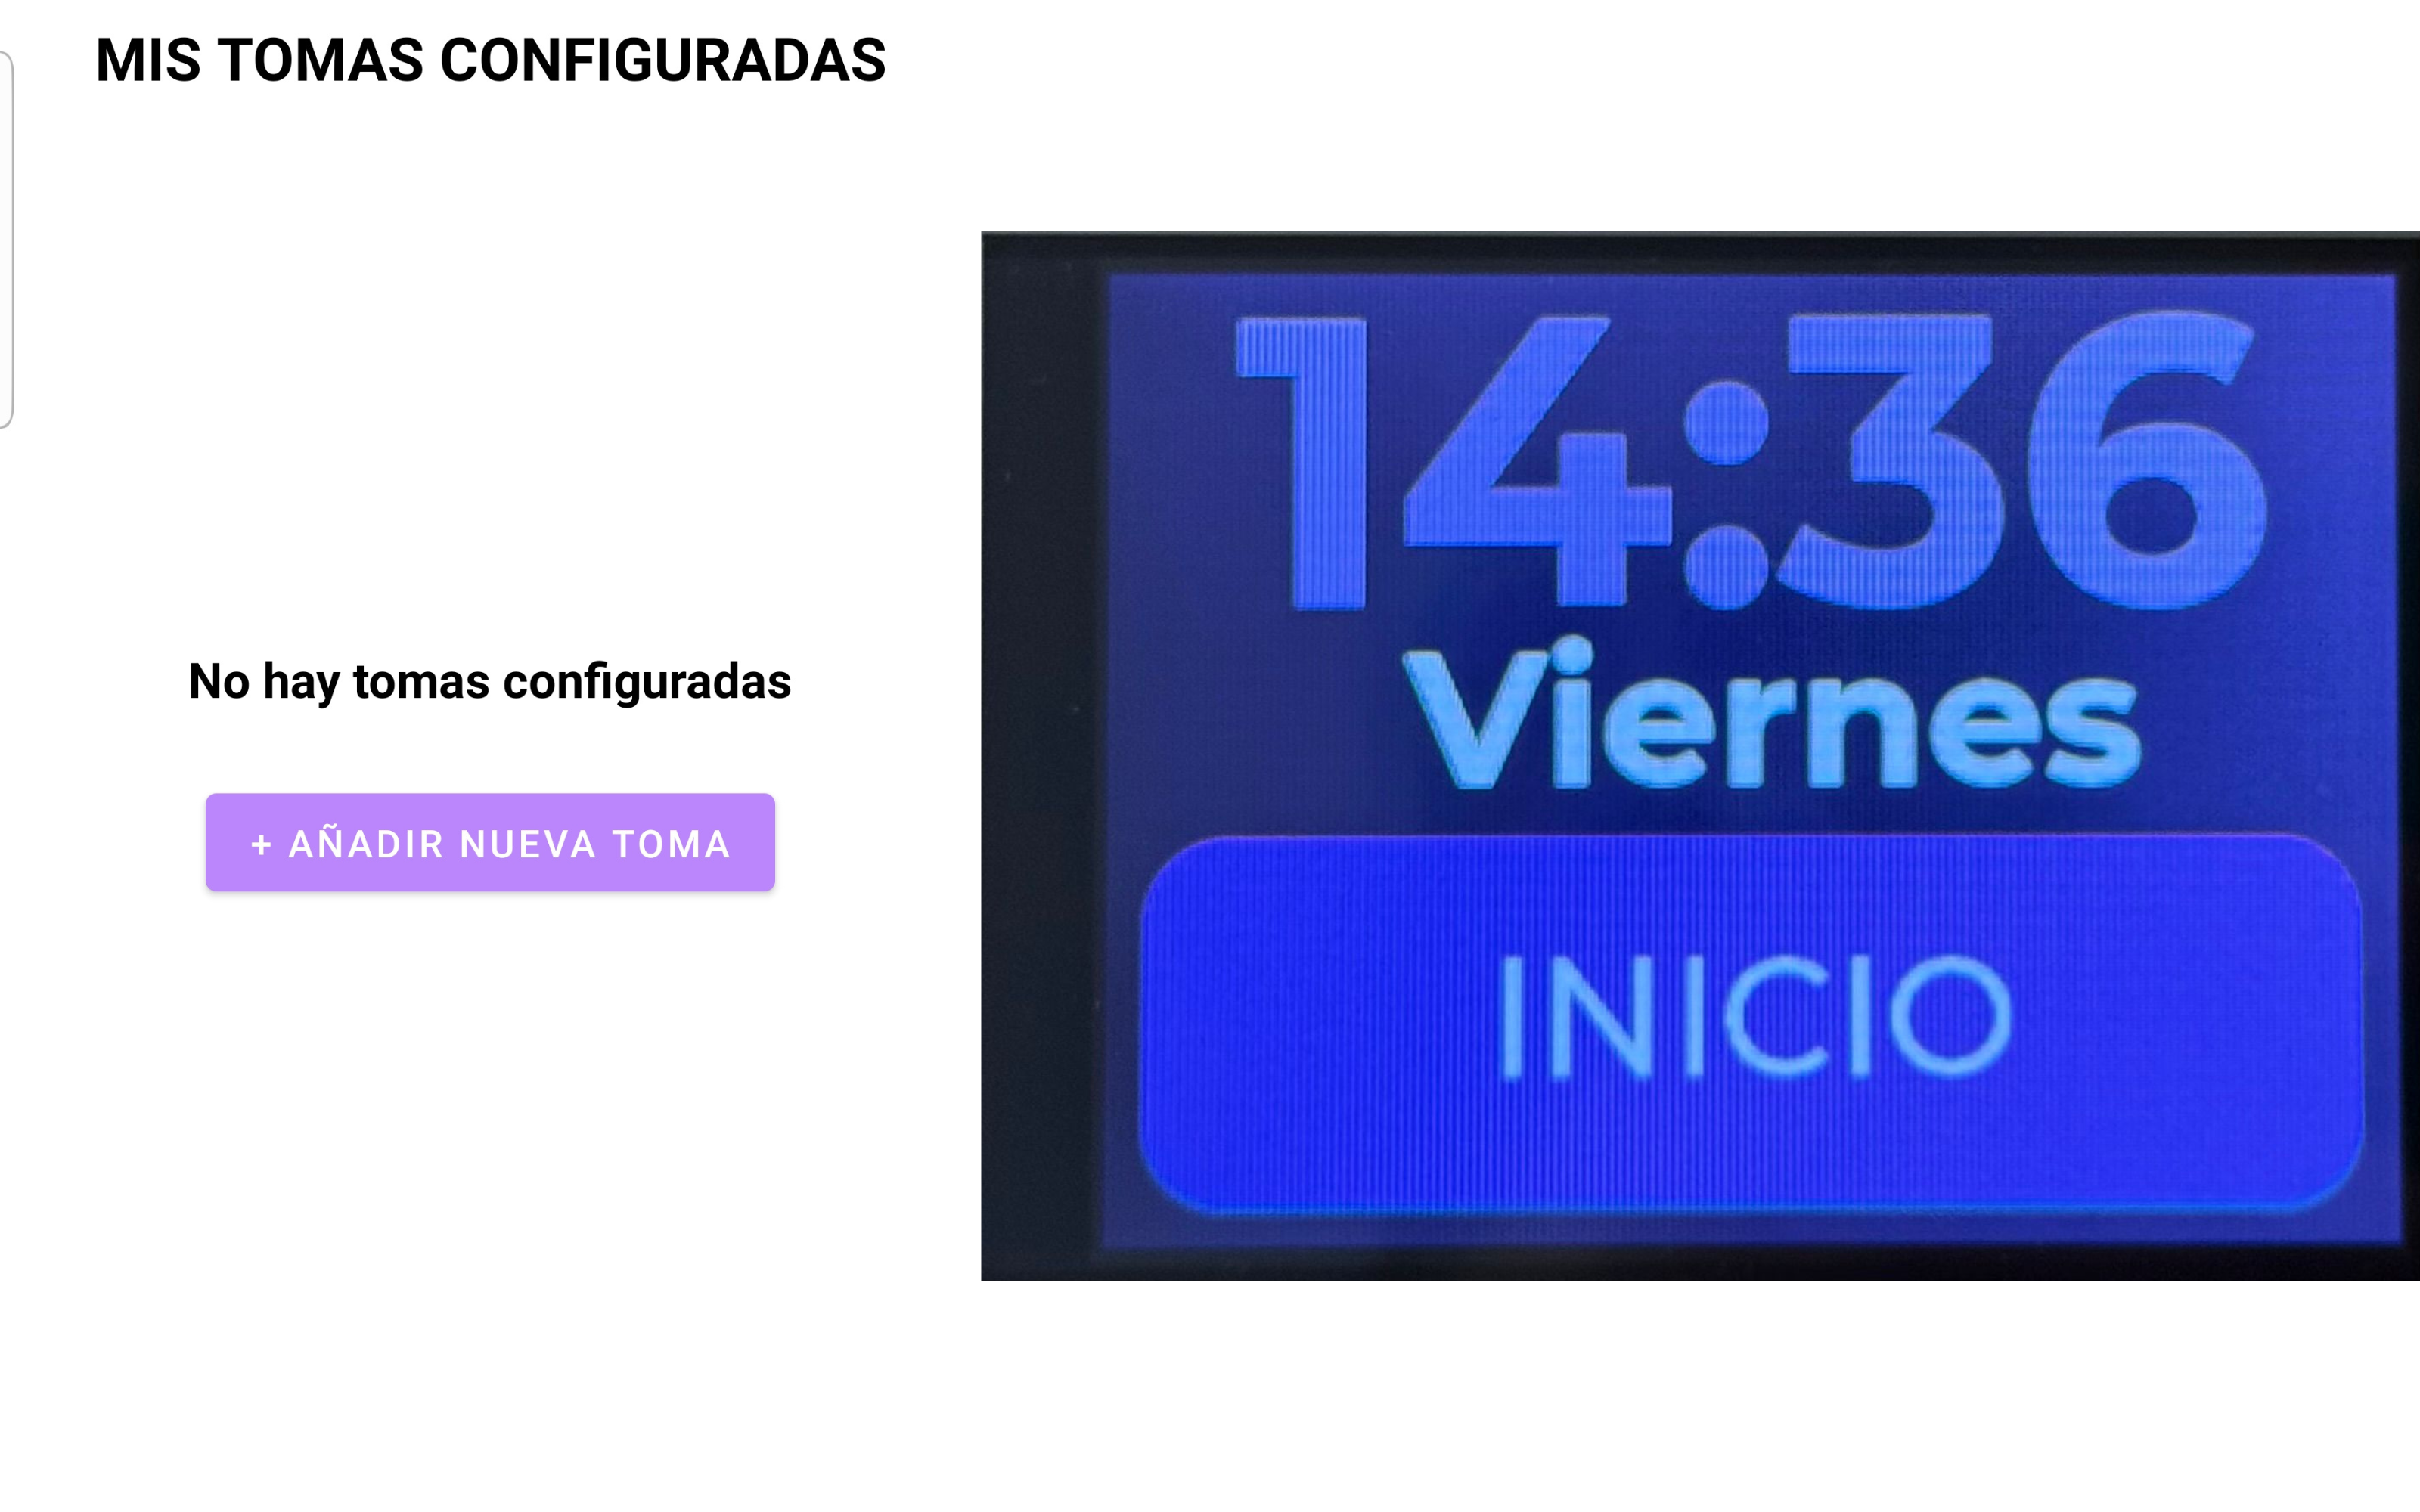
\includegraphics[width=0.85\textwidth]{figs/collage_paso7_conf.png}
    \caption{Pantallas que aparecen tras finalizar la sincronización}
    \label{fig:collage_paso7_conf}
\end{figure}

\section{Gestión de tomas}

Las tomas de medicación pueden gestionarse tanto desde la aplicación móvil como desde el propio dispositivo.\\

Antes de pasar a configurar tomas, asegúrese de introducir los medicamentos que quiere usar en el apartado de `MEDICAMENTOS` de la app. Seleccionando añadir medicamento podrá añadir los nombres o eliminarlo si ya no lo quiere tener registrado.

\begin{figure}[H]
    \centering
    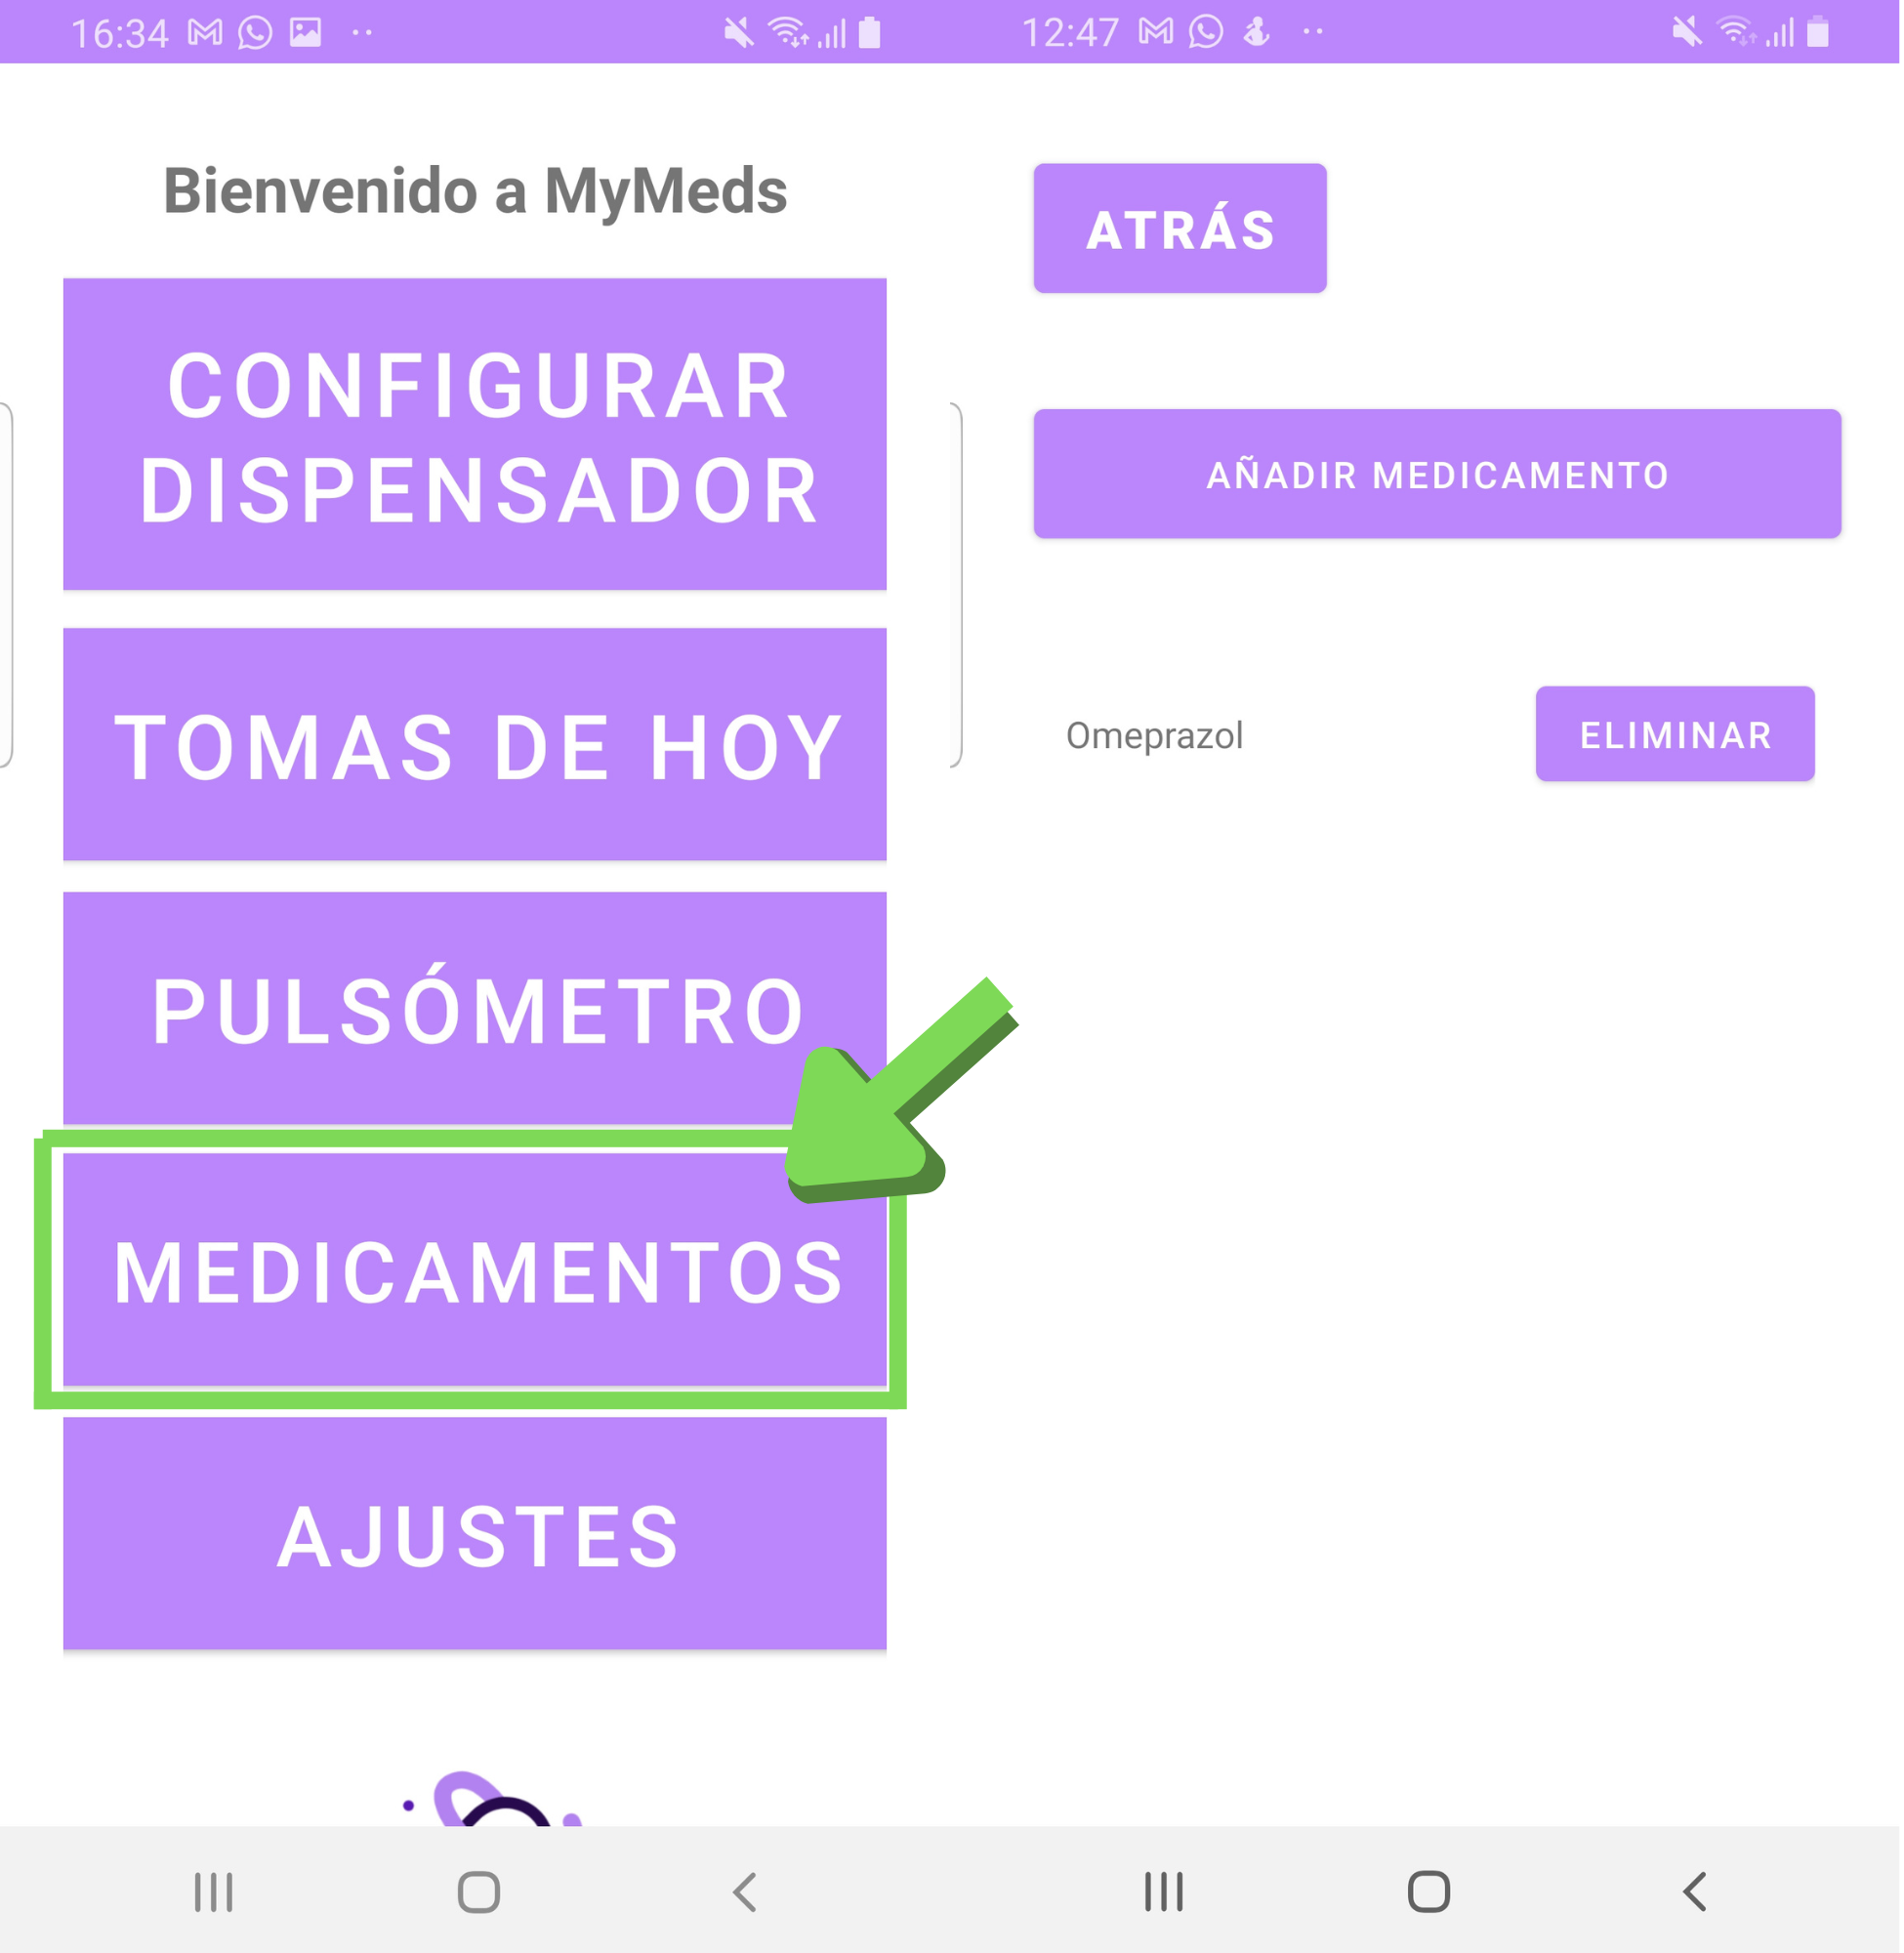
\includegraphics[width=0.75\textwidth]{figs/medicamentos_manual.png}
    \caption{Registro de los medicamentos}
    \label{fig:medicamentos_manual}
\end{figure}

\subsection{Añadir una toma}

Para crear una nueva toma:

\begin{itemize}
\item Pulsar el botón \textit{Añadir toma}.
\item Seleccionar la hora de la toma.
\item Elegir los días de repetición.
\item Escoger la medicación del desplegable.
\item Activar o desactivar el recordatorio asociado.
\item Opcionalmente, seleccionar el número de minutos de antelación para un aviso previo.
\item Guardar la configuración.
\end{itemize}

\begin{figure}[H]
    \centering
    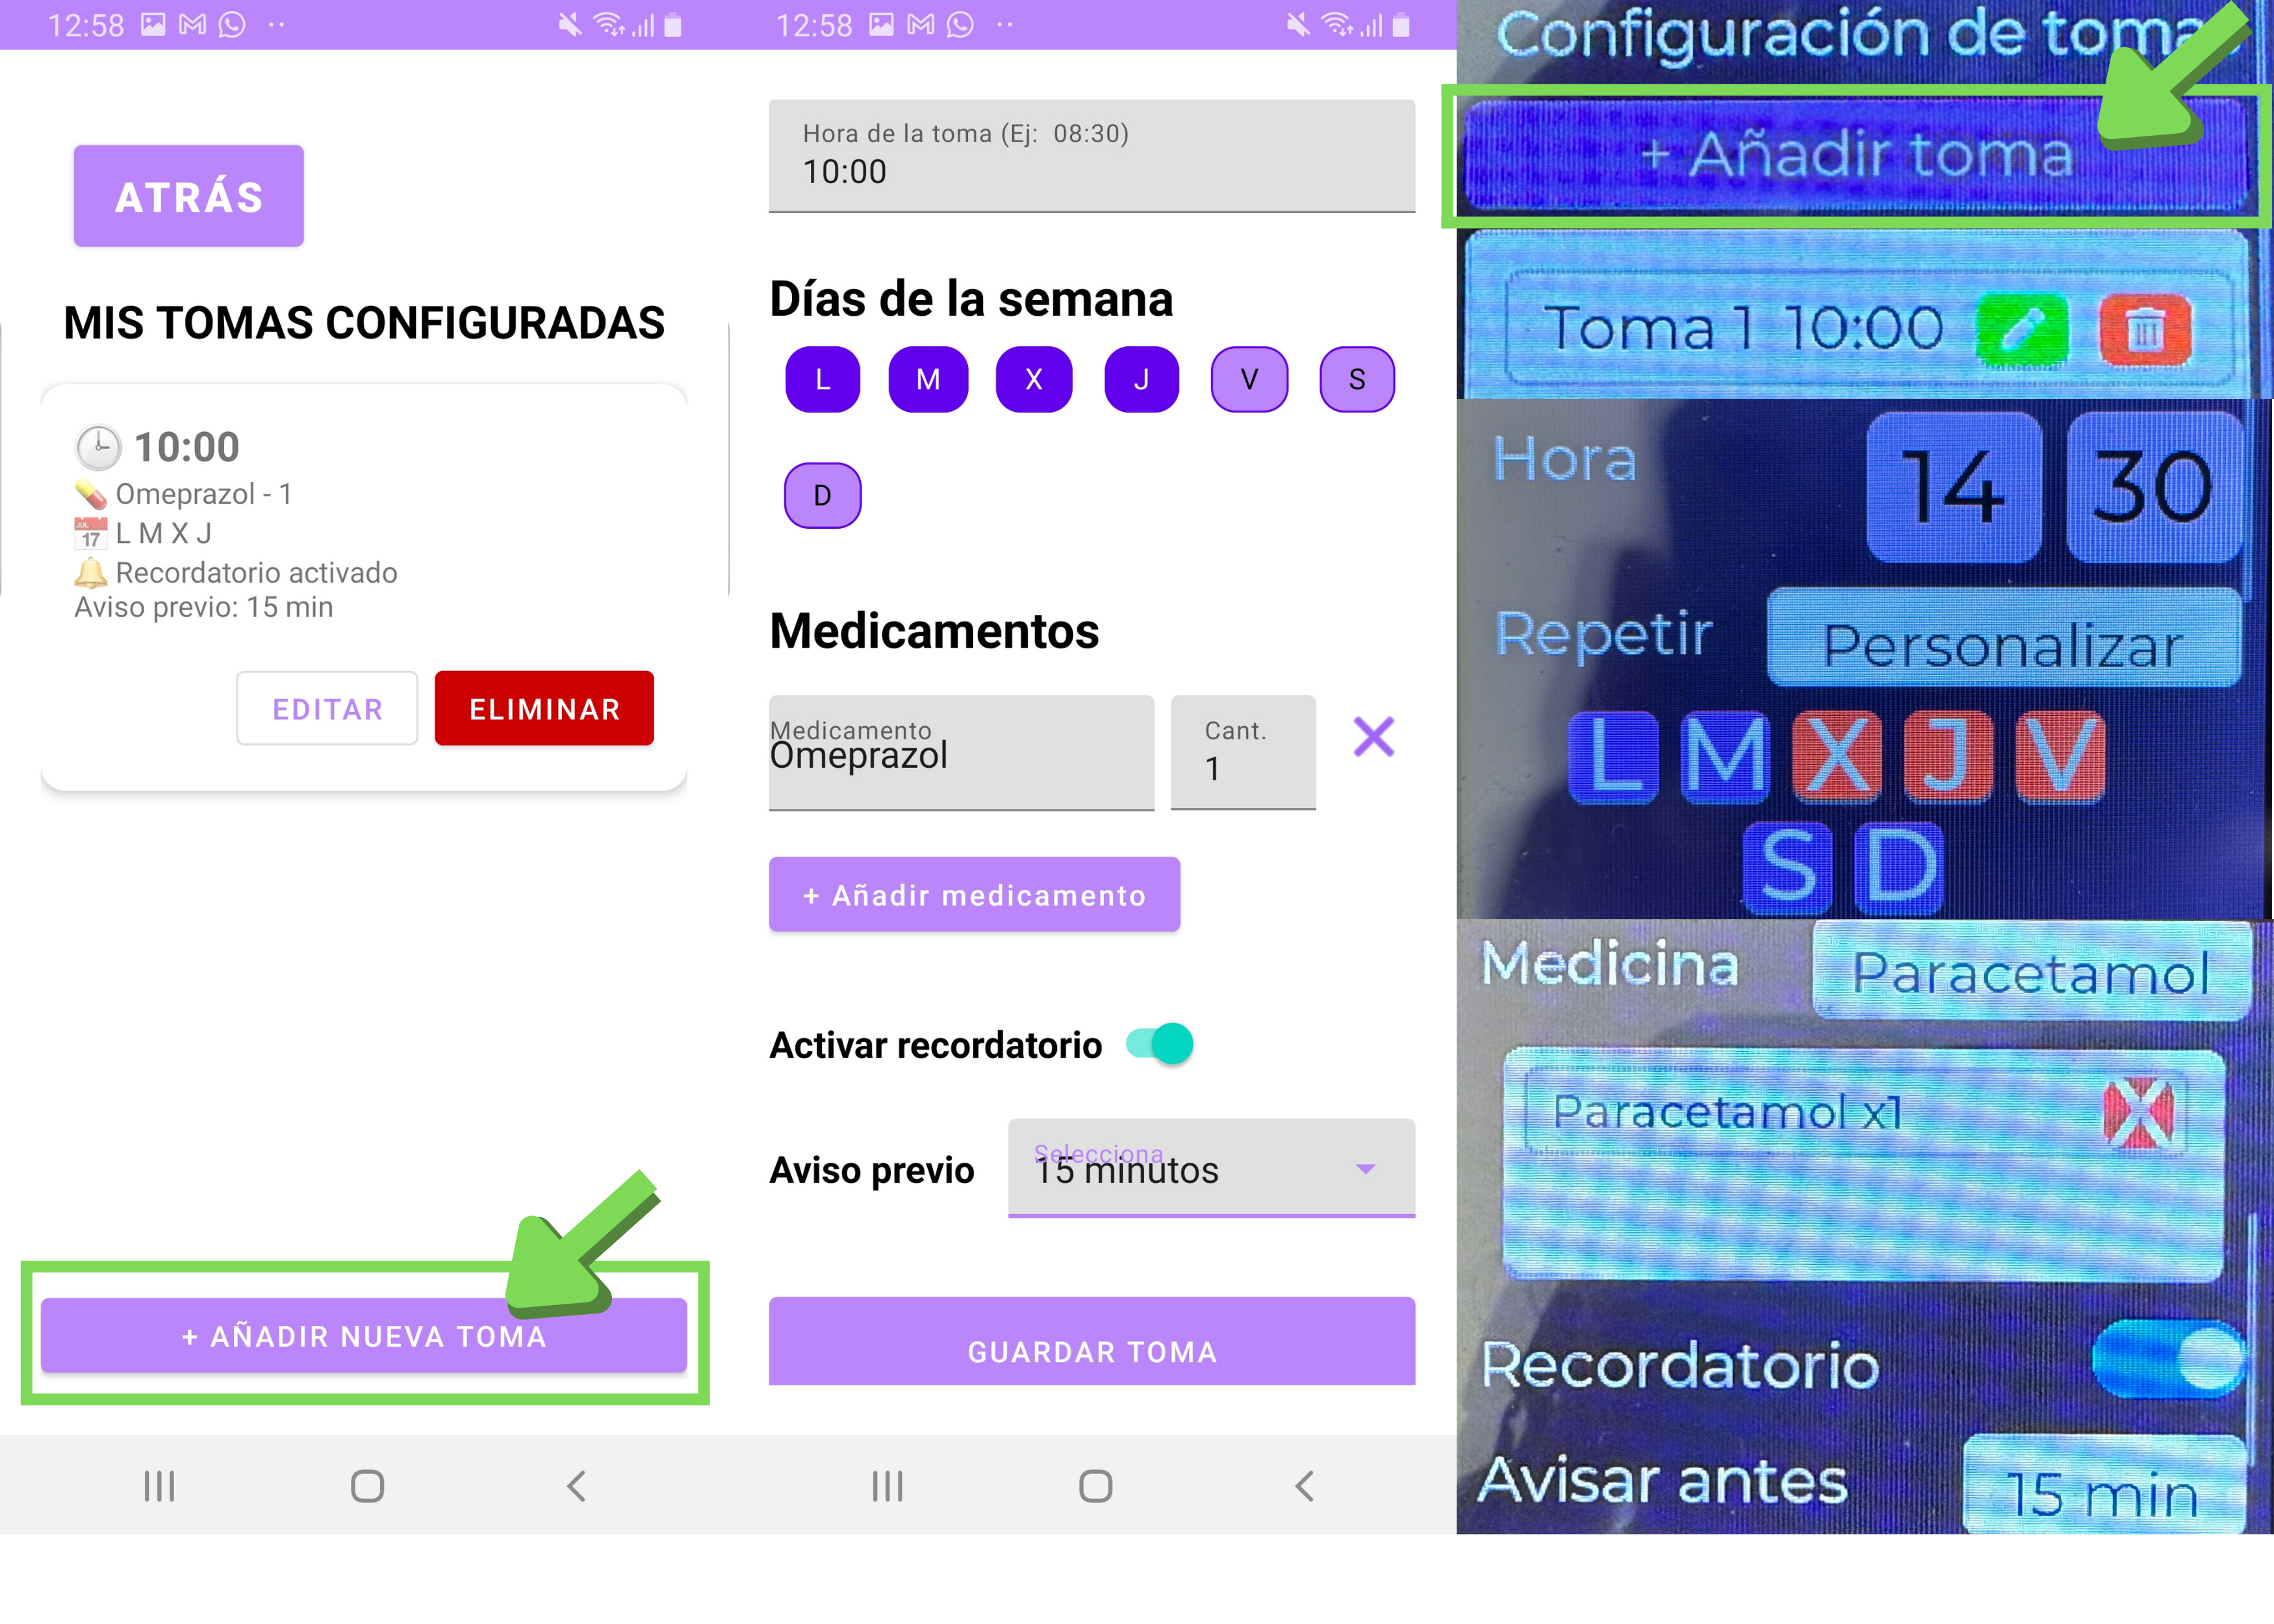
\includegraphics[width=0.85\textwidth]{figs/añadir_toma_manual.png}
    \caption{Añadir tomas en ambos dispositivos}
    \label{fig:añadir_toma_manual}
\end{figure}

\subsection{Editar una toma}

Para modificar una toma existente, seleccionar la opción \textit{Editar} correspondiente a la toma deseada.

Es posible modificar:

\begin{itemize}
\item La hora programada.
\item Los días de repetición.
\item El estado del recordatorio.
\item El tiempo de aviso previo.
\item La medicación asociada a la toma.
\end{itemize}

\begin{figure}[H]
    \centering
    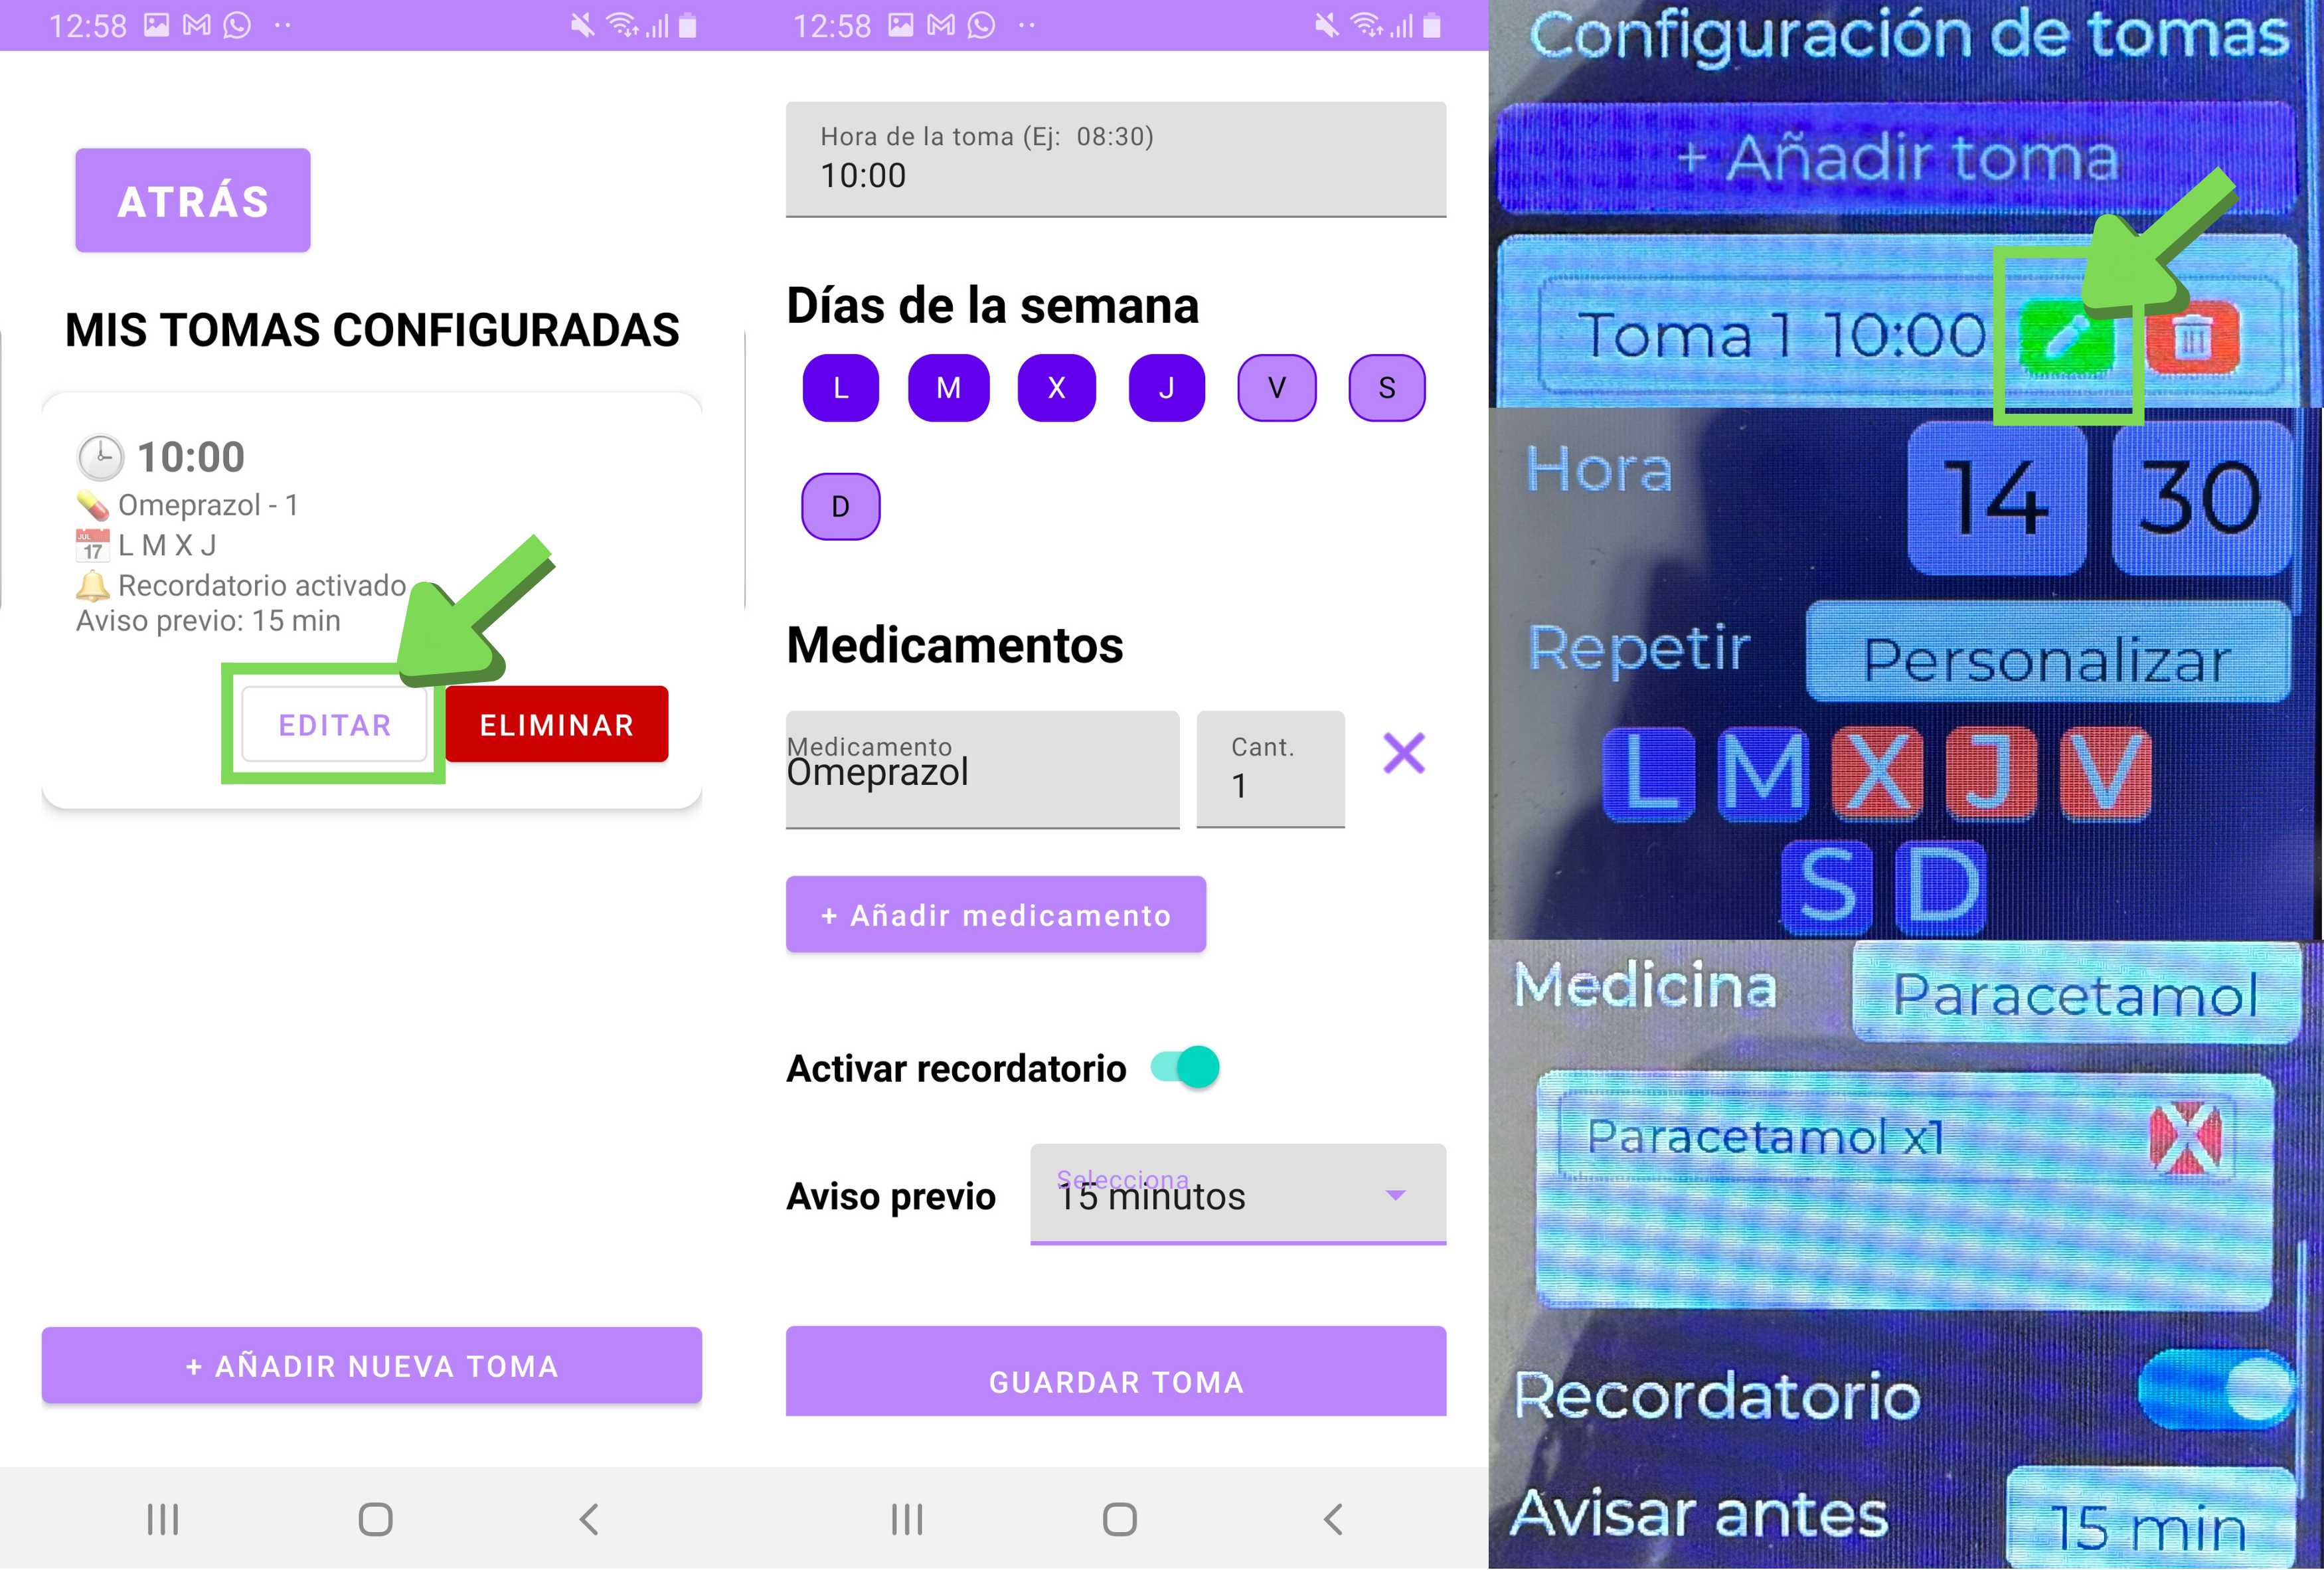
\includegraphics[width=0.85\textwidth]{figs/editar_toma_manual.png}
    \caption{Editar tomas en ambos dispositivos}
    \label{fig:editar_toma_manual}
\end{figure}

\subsection{Eliminar una toma}

Para eliminar una toma, seleccionar la opción \textit{Eliminar} correspondiente a la toma deseada. El sistema mostrará un mensaje de confirmación antes de realizar la eliminación definitiva.

\begin{figure}[H]
    \centering
    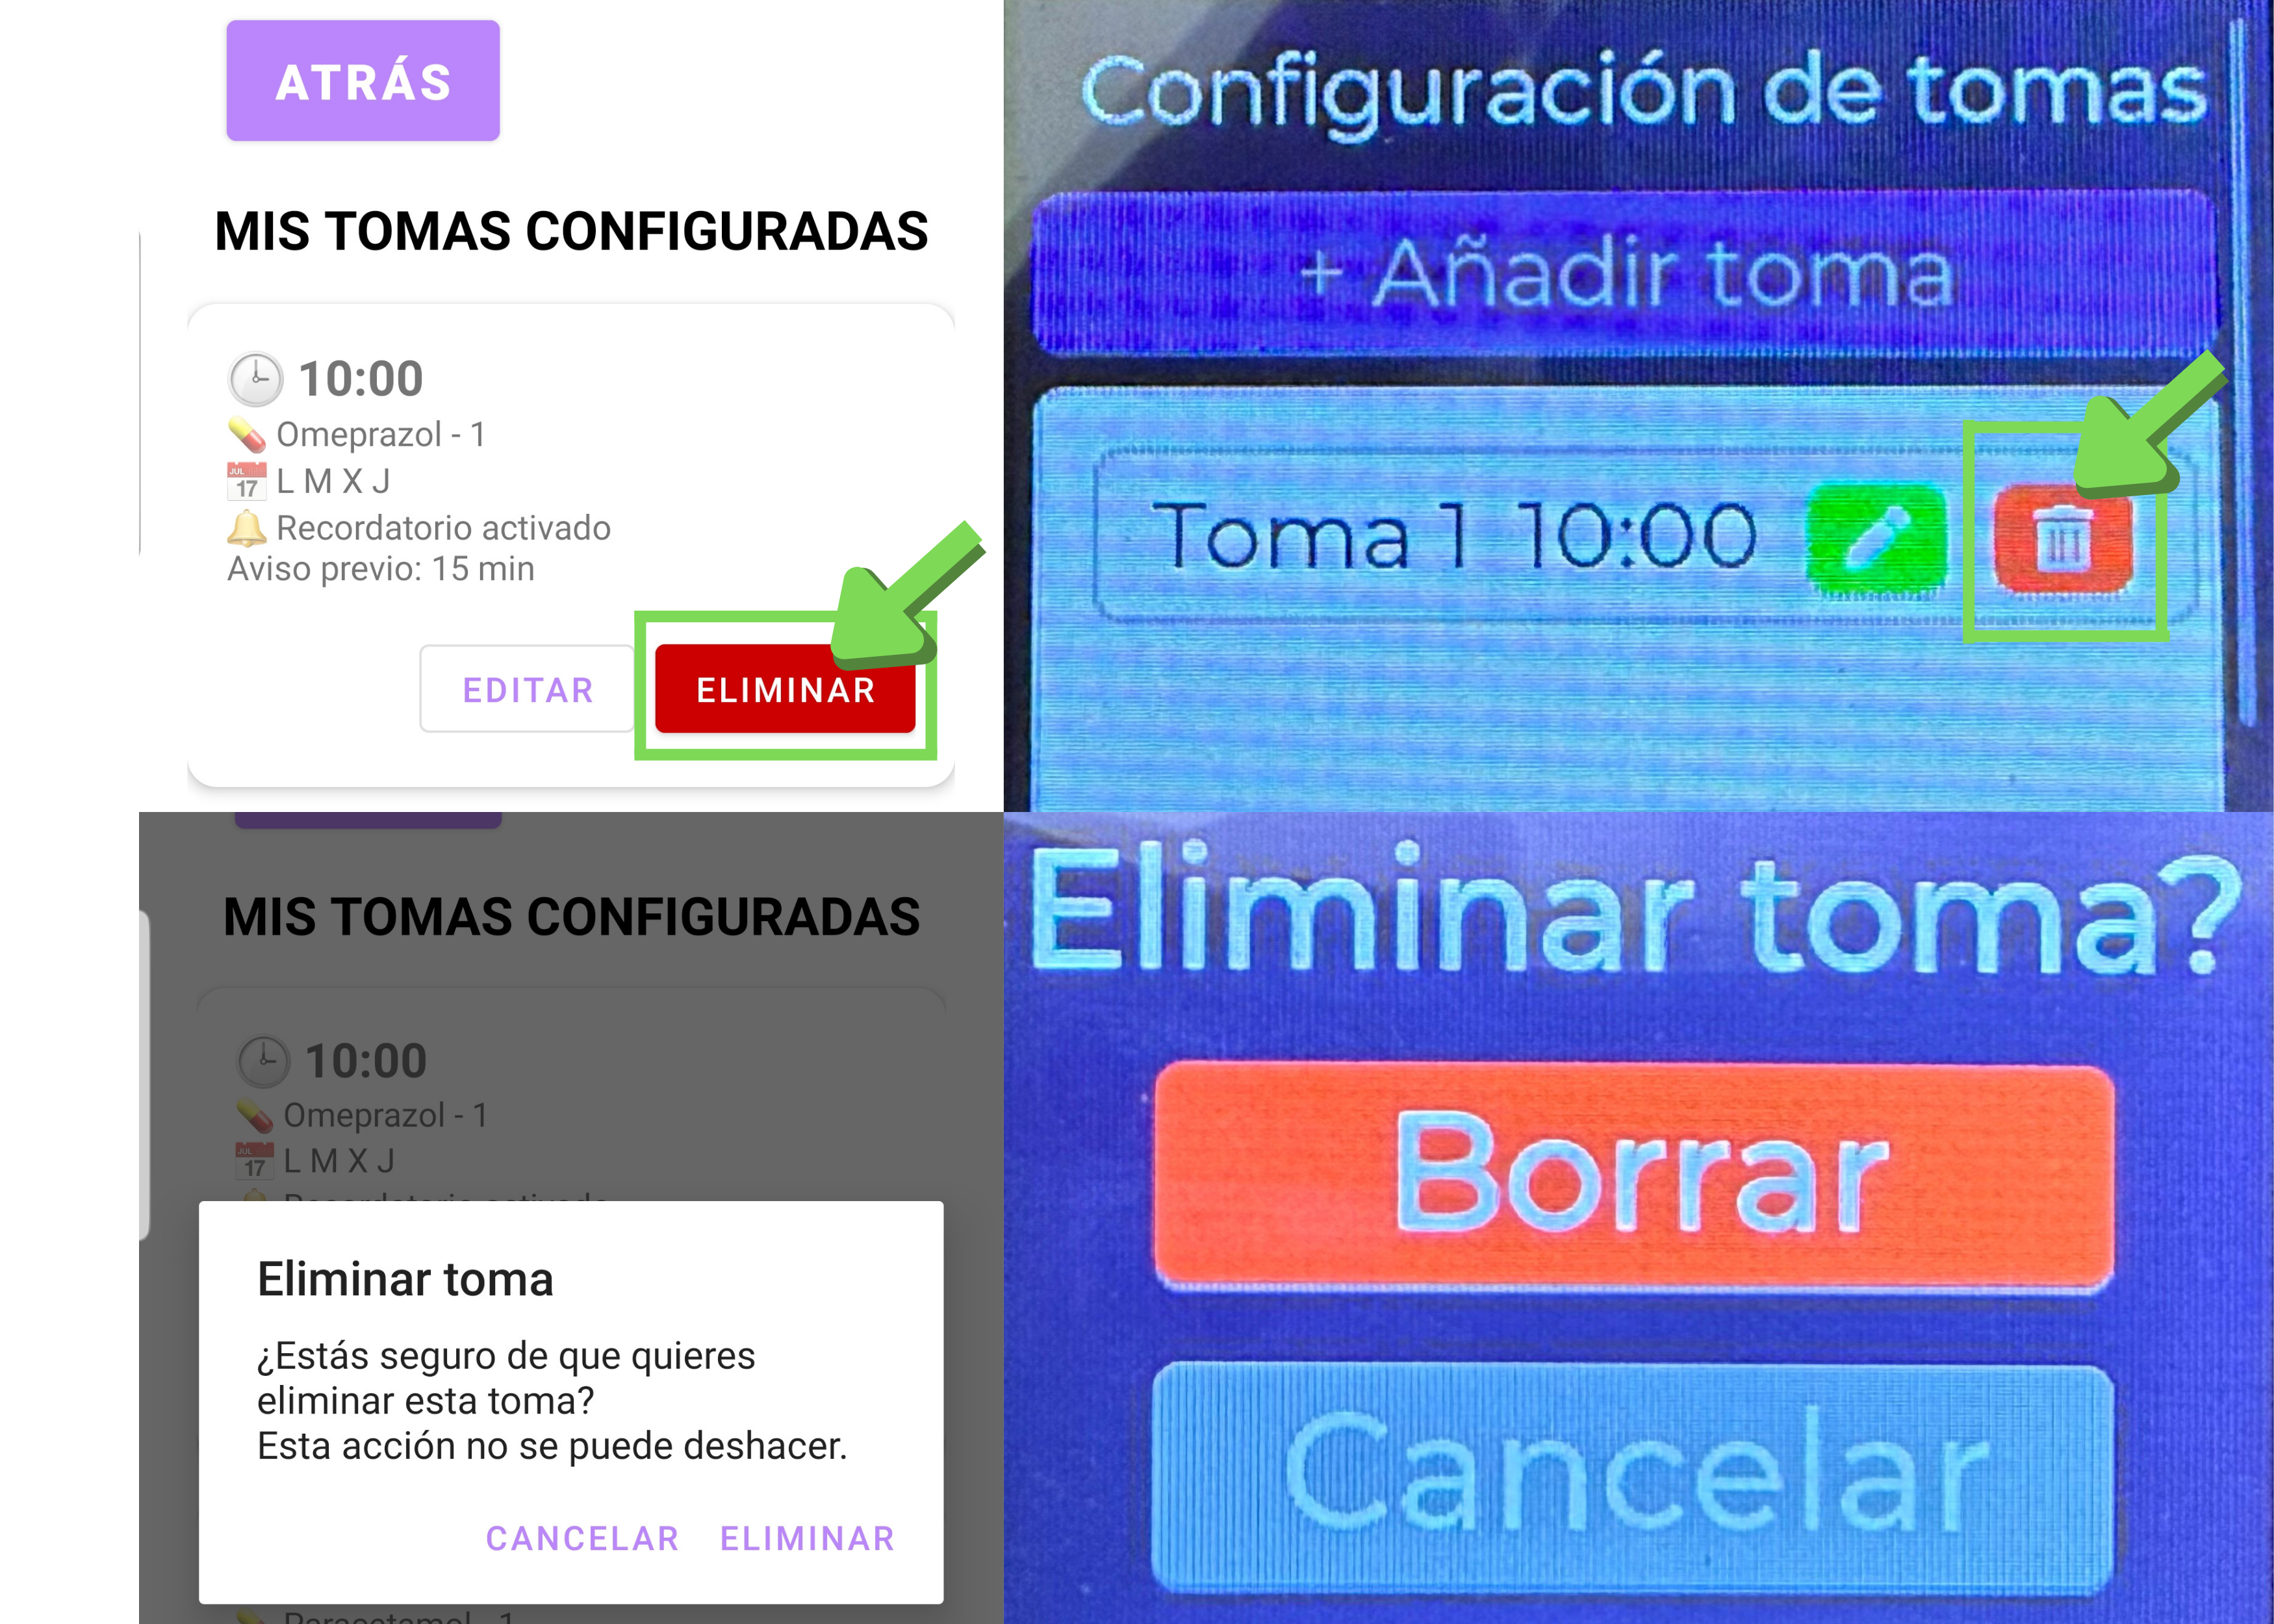
\includegraphics[width=0.85\textwidth]{figs/eliminar_toma_manual.png}
    \caption{Eliminar tomas en ambos dispositivos}
    \label{fig:eliminar_toma_manual}
\end{figure}

\subsection{Sincronización}

Todas las modificaciones realizadas desde la aplicación móvil se sincronizan automáticamente con el dispositivo y viceversa.\\

Durante el proceso de sincronización se actualizan las tomas, los medicamentos asociados y el resto de configuración almacenada.\\

El sistema no realiza actualizaciones parciales, sino que reemplaza la configuración anterior por la nueva información sincronizada.

\section{Funcionamiento del sistema}

Una vez configurado, el dispositivo almacena la información necesaria en su memoria interna y puede funcionar de forma autónoma.\\

El sistema comprueba continuamente la fecha y la hora actuales para determinar si existe alguna toma programada.\\

Cuando llega el momento de una toma:

\begin{itemize}
\item Se activa una señal acústica.
\item Se muestra un aviso en pantalla.
\item Se realiza automáticamente la dispensación correspondiente.
\end{itemize}

Gracias al almacenamiento local, el funcionamiento del dispositivo no depende de mantener una conexión permanente con la aplicación móvil.

\section{Funcionamiento sin conexión con la App}

Una vez sincronizado, el dispositivo puede continuar funcionando sin necesidad de comunicación con la aplicación móvil. Además, si se abre la aplicación se sincronizan los datos de ambos.

\begin{itemize}
\item Conserva las tomas almacenadas.
\item Mantiene la configuración previamente sincronizada.
\item Continúa realizando las dispensaciones programadas.
\item Sigue mostrando la información disponible en pantalla.
\end{itemize}

Si el dispositivo pierde la alimentación eléctrica, la configuración permanecerá almacenada y no será necesario repetir el proceso de vinculación.\\

Únicamente será necesario realizar una nueva configuración si se eliminan los datos almacenados en la aplicación o si se restablece la memoria interna del dispositivo.

\section{Pulsómetro e historial de mediciones}

El dispositivo incorpora un sensor biomédico capaz de estimar la frecuencia cardíaca del usuario.\\

Para realizar una medición:

\begin{itemize}
\item Acceder al apartado \textit{Pulsómetro} desde la pantalla principal.
\item Colocar el dedo sobre el sensor.
\item Mantener el dedo inmóvil durante el proceso de medición.
\item Esperar a que finalice la adquisición de datos.
\item Consultar el resultado mostrado en pantalla.
\end{itemize}

\begin{figure}[H]
    \centering
    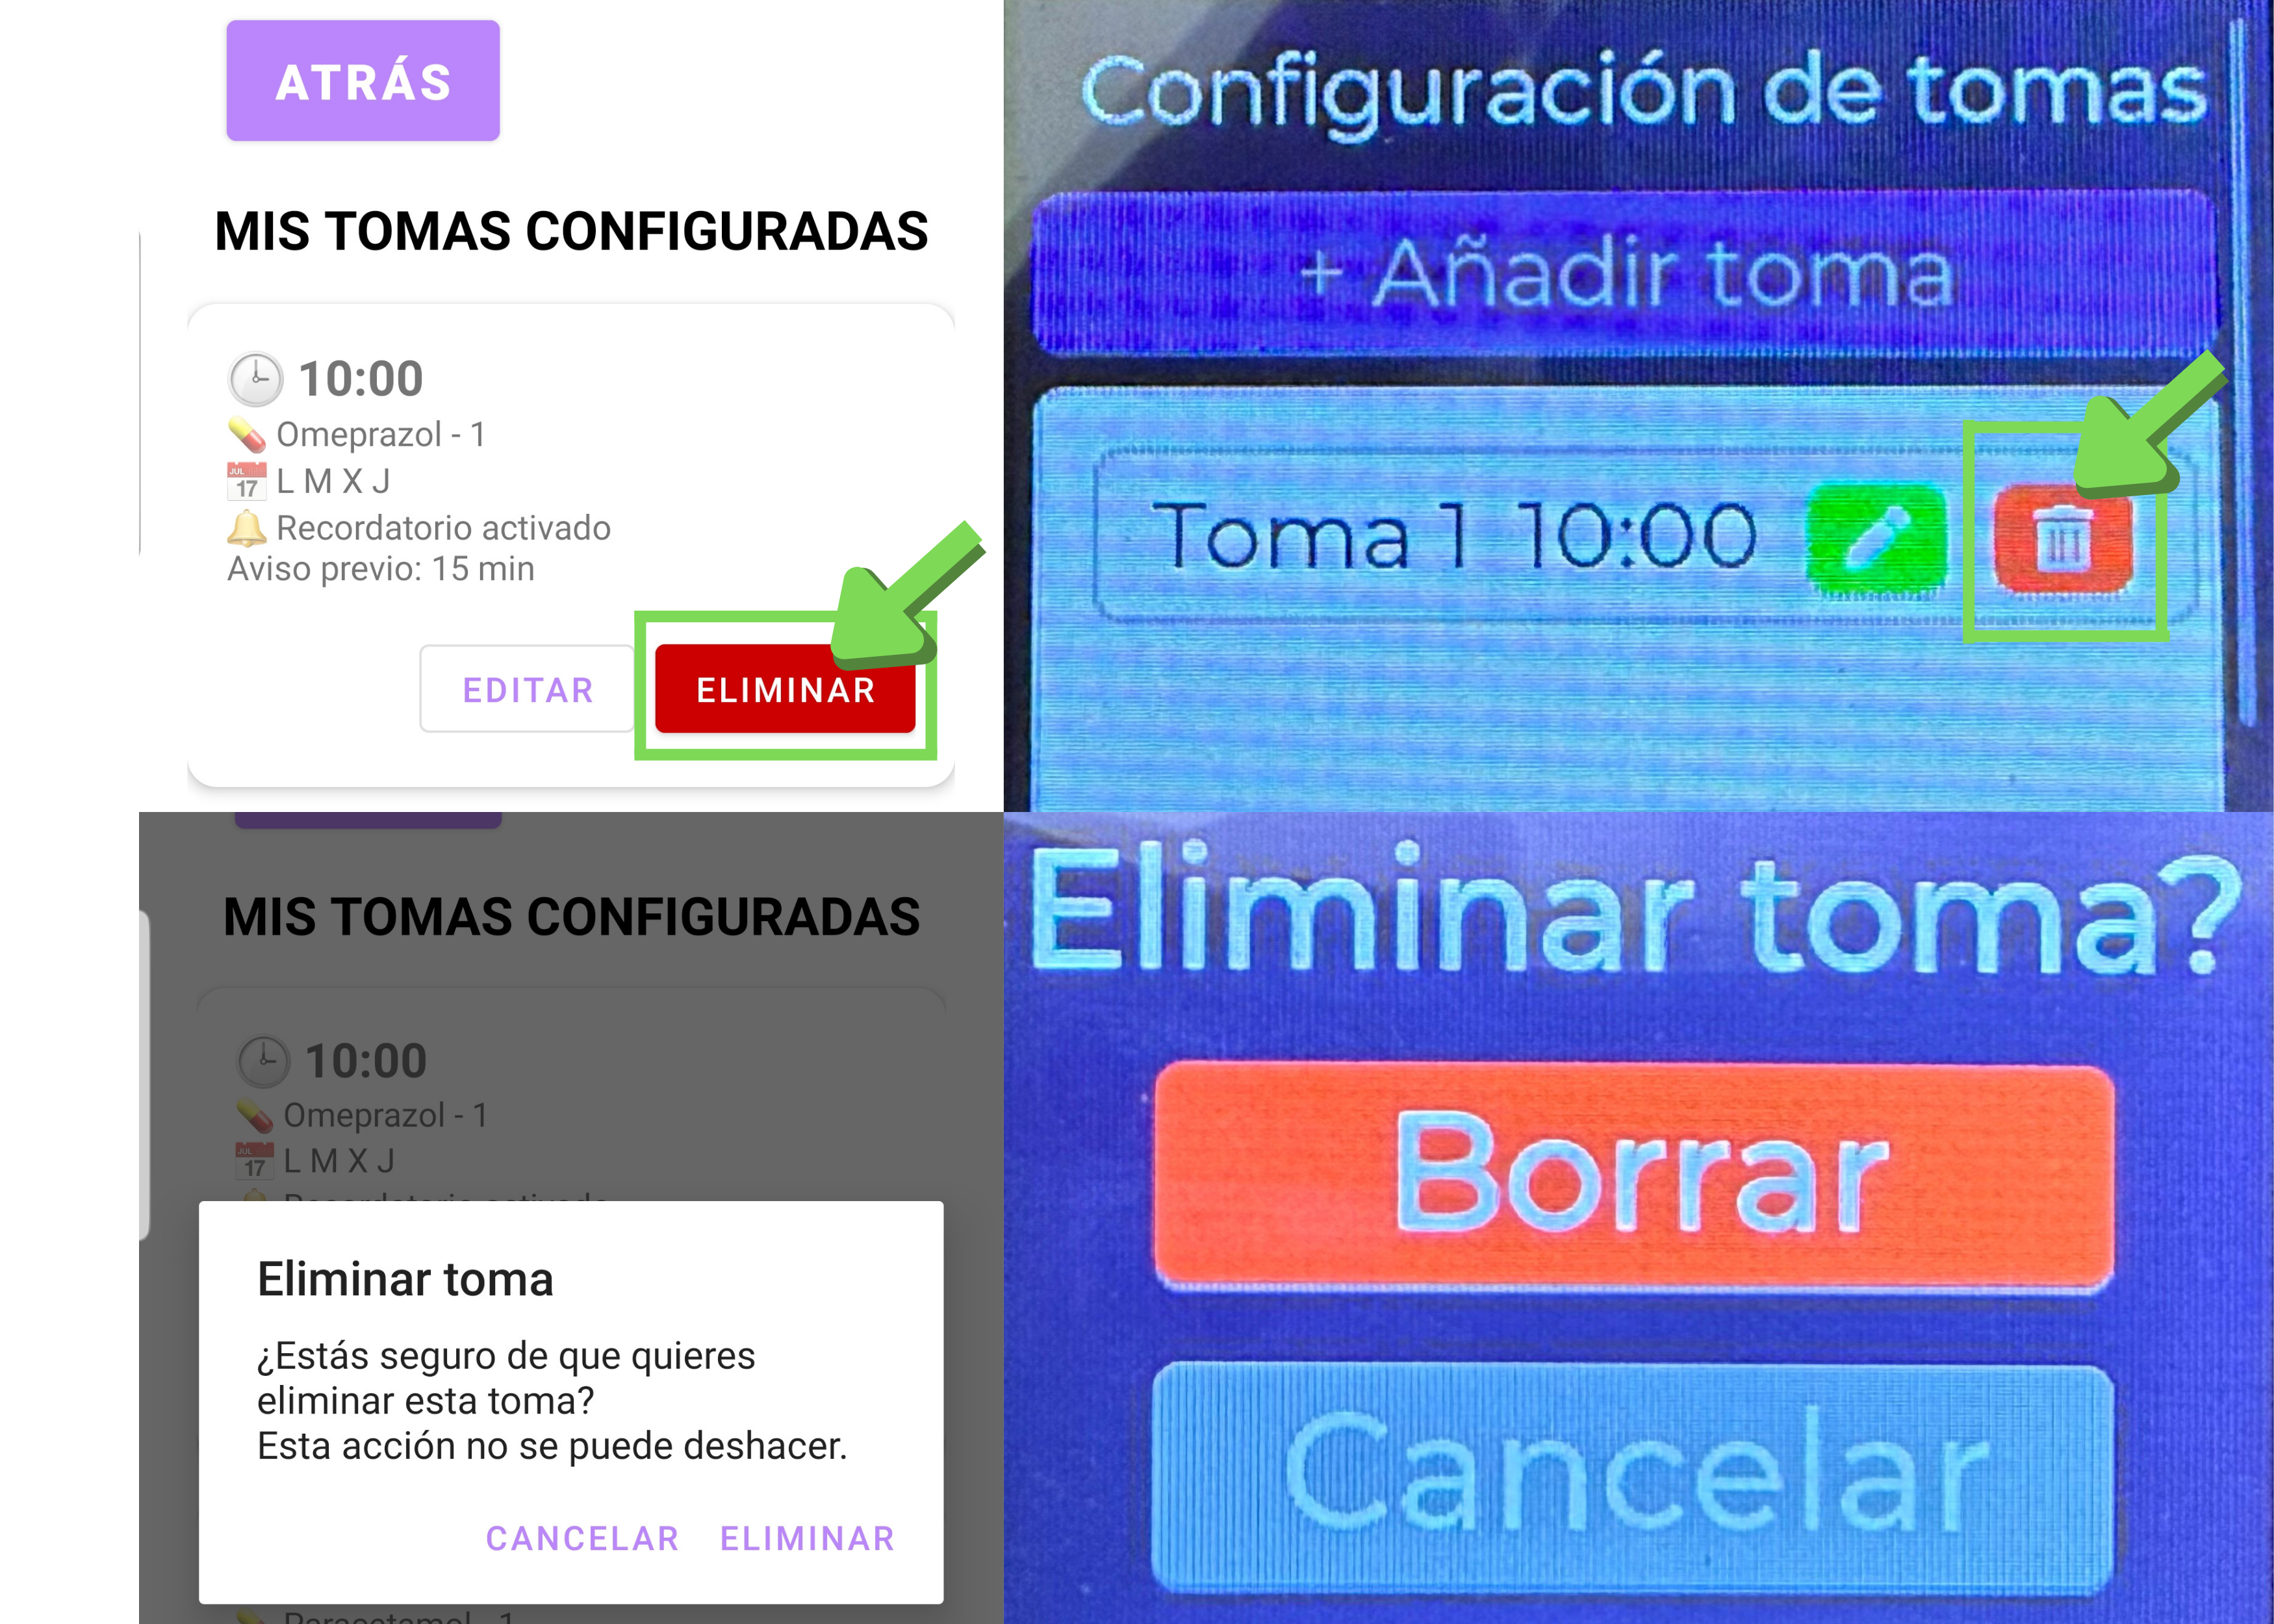
\includegraphics[width=0.85\textwidth]{figs/eliminar_toma_manual.png}
    \caption{Eliminar tomas en ambos dispositivos}
    \label{fig:paso4_conf}
\end{figure}

Durante la medición se mostrará el progreso de adquisición de muestras necesarias para el cálculo de la frecuencia cardíaca.\\

Las mediciones realizadas se almacenan localmente en la tarjeta microSD del dispositivo, permitiendo consultar un histórico básico directamente desde el dispensador.\\

Adicionalmente, las mediciones se sincronizan con la aplicación móvil, donde es posible acceder al historial completo, realizar búsquedas, visualizar gráficas y generar informes.\\

\textbf{Importante:} Las mediciones proporcionadas por el sistema tienen carácter orientativo y no sustituyen a un dispositivo médico profesional ni al criterio de un profesional sanitario.

\section{Recomendaciones de uso}

Para un correcto funcionamiento:

\begin{itemize}
\item Mantén el dispositivo en un entorno limpio y seco
\item Evita golpes o caídas
\item Utiliza una fuente de alimentación adecuada 5V/3A
\item Revisa periódicamente el estado del dispensador
\end{itemize}

\section{Problemas frecuentes}

\textbf{El dispositivo no enciende}
Comprueba la conexión del cable USB-C.\\

\textbf{No aparecen las tomas}
Realiza una modificación en la aplicación para forzar la sincronización.\\

\textbf{El dispositivo no tiene configuración}
Vuelve a sincronizar desde la aplicación móvil.\\

\textbf{No se escucha el aviso}
Verifica el funcionamiento del altavoz.\\

\textbf{No conecta al WiFi}
Reinicia el dispositivo e introduce de nuevo los datos de la red.\\

\section{Información adicional}

El sistema ha sido diseñado para ofrecer una experiencia sencilla, intuitiva y accesible, especialmente orientada a usuarios que requieren apoyo en la gestión de su medicación diaria.\\

La combinación del dispositivo y la aplicación permite una gestión completa, automatizada y fiable de las tomas.
